% !TEX program = lualatex
% Tema 4, parte I: mismo contenido que la versión anterior; sólo cambia el formato.
\documentclass[11pt,twoside]{article}
\usepackage{apuntes-oscuro}

\asignatura{Ecuaciones Diferenciales}
\cabecera{Tema 4\ \ ·\ \ EDO lineales de orden superior}
\hypersetup{pdftitle={Tema 4. Parte I. Estructura de las soluciones y funciones de Green},
  pdfauthor={Daniel Martín Guerrero}}

% ---------- notación propia del tema ----------
\newcommand\Lop{\mathcal L}
\newcommand\yh{\hat y}
\newcommand\vyh{\hat{\bm y}}
\newcommand\Cl{\mathcal C}
\newcommand\vk{\bm k}
\newcommand\vc{\bm c}
\newcommand\vb{\bm b}
\newcommand\ve{\bm e}
\newcommand\vK{\bm K}
\newcommand\vgamma{\bm\gamma}
\newcommand\abs[1]{\lvert#1\rvert}
\newcommand\mat[1]{\begin{pmatrix}#1\end{pmatrix}}
\newcommand\smat[1]{\left(\begin{smallmatrix}#1\end{smallmatrix}\right)}
\newcommand\xt{\tilde x}
\newcommand\gen[1]{\langle#1\rangle}
\usetikzlibrary{decorations.pathmorphing}

\begin{document}

% =====================================================================
%  PORTADA
% =====================================================================
\begin{titlepage}
\thispagestyle{empty}
\centering
\vspace*{-0.6cm}

\includegraphics[width=4.6cm]{figuras/usal.png}\par
\vspace{0.75cm}
{\color{sky}\rule{\textwidth}{0.5pt}}\par
\vspace{0.55cm}
{\color{muted}\small\textls[220]{\textsc{Facultad de Ciencias}}\quad·\quad\textls[220]{\textsc{Grado en Física}}}\par
\vspace{1.25cm}
{\color{acc}\textls[260]{\textsc{Ecuaciones Diferenciales}}}\par
\vspace{0.2cm}
{\color{muted}\small\textls[260]{\textsc{Tema 4\ \ ·\ \ Parte I}}}\par
\vspace{1.25cm}
{\fontsize{27}{33}\selectfont\bfseries EDO lineales de orden superior\par}
\vspace{0.12cm}
{\fontsize{19}{24}\selectfont\bfseries núcleo, wronskiano y funciones de Green\par}
\vspace{0.55cm}
{\color{acc}\rule{2.4cm}{0.8pt}}\par
\vspace{0.45cm}
{\color{muted}\small\itshape Operador lineal\quad·\quad Sistema fundamental y wronskiano\quad·\quad Coeficientes constantes\par
Raíces múltiples\quad·\quad Variación de las constantes\quad·\quad Funciones de Green\par}
\vspace{0.45cm}
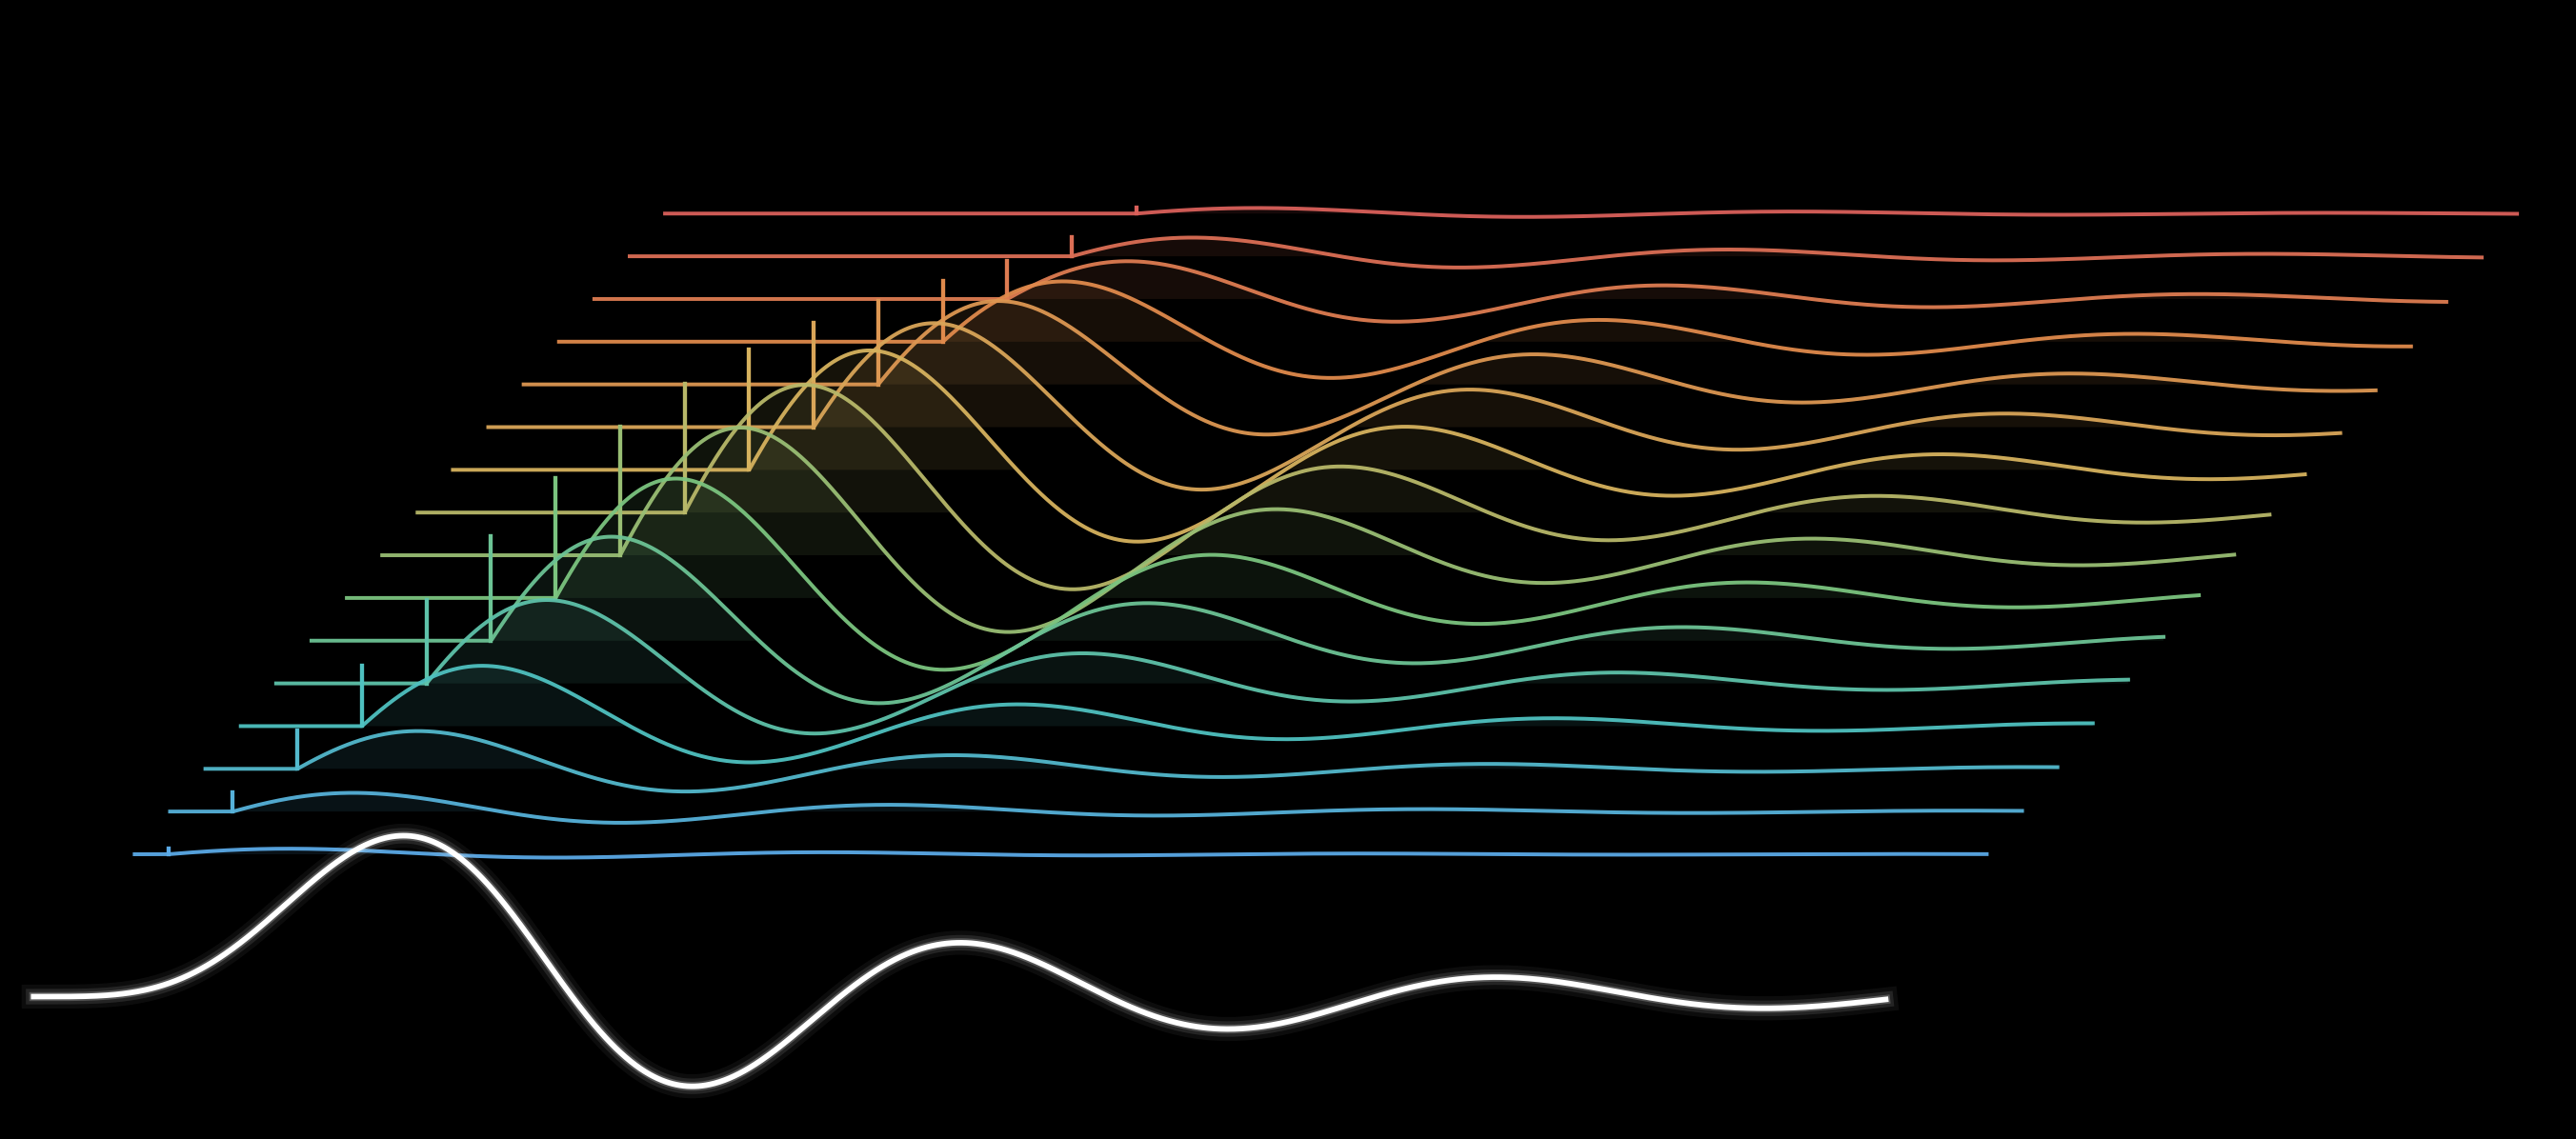
\includegraphics[width=0.86\textwidth]{figuras/portada_t4p1.png}\par
\vspace{0.35cm}
{\small$\displaystyle \Lop_x\,G(x,\xt)=\delta(x-\xt),\qquad y_p(x)=\int G(x,\xt)\,b(\xt)\,\dd\xt$\par}
\vfill
{\color{sky}\rule{\textwidth}{0.5pt}}\par
\vspace{0.3cm}
\begin{minipage}[t]{0.32\textwidth}\raggedright
{\color{acc}\footnotesize\textls[200]{\textsc{Autor}}}\par\vspace{2pt}
{\small Daniel Martín Guerrero}
\end{minipage}\hfill
\begin{minipage}[t]{0.32\textwidth}\centering
{\color{acc}\footnotesize\textls[200]{\textsc{Profesorado}}}\par\vspace{2pt}
{\small Pilar García Estévez\\ José Beltrán Jiménez\\ María Pérez Garrote}
\end{minipage}\hfill
\begin{minipage}[t]{0.32\textwidth}\raggedleft
{\color{acc}\footnotesize\textls[200]{\textsc{Apuntes formalizados}}}\par\vspace{2pt}
{\small Salamanca, curso 2026/2027}\\[1pt]
{\footnotesize\color{muted}Teoría y ejemplos resueltos}
\end{minipage}
\end{titlepage}

% =====================================================================
%  ÍNDICE
% =====================================================================
\setcounter{page}{2}
{\hypersetup{linkcolor=fg}\tableofcontents}
\clearpage

% =====================================================================
\section{Planteamiento y estructura de la solución}\label{sec:planteamiento}
% =====================================================================

\begin{motivacion}{Resumen}
Estudiamos la ecuación lineal de orden $n$ $\Lop[y]=a_n(x)\,y^{(n)}+\dots+a_0(x)\,y=b(x)$. Toda la teoría descansa en
la linealidad de $\Lop$: de ella se siguen que las soluciones de la homogénea forman un espacio vectorial de dimensión
$n$ ---lo que demostramos identificándolo con el espacio de datos iniciales--- y que la solución general es la suma de
la homogénea y una particular. Para coeficientes constantes construimos una base del núcleo factorizando $\Lop$ como
polinomio en $D=\dd/\dd x$, incluido el caso de raíces múltiples, que resolvemos con un lema de conjugación por la
exponencial. Para la particular deducimos la fórmula matricial de variación de las constantes y mostramos que coincide
con el método de la función de Green, la respuesta del sistema a un impulso unitario, que permite escribir la solución
como superposición de respuestas a fuentes puntuales.

\smallskip
\textcolor{acc}{\textsc{Palabras clave.}} operador lineal, sistema fundamental, wronskiano, polinomio característico,
raíces múltiples, variación de las constantes, función de Green, delta de Dirac, causalidad.

\smallskip
\textcolor{acc}{\textsc{MSC 2020.}} 34A30, 34A05, 34B27.
\end{motivacion}

Todo el tema descansa sobre una sola propiedad: el operador diferencial es lineal. De ella se siguen tres hechos: que la
solución general es «homogénea más particular», que las soluciones de la homogénea forman un espacio vectorial de
dimensión $n$, y que una fuente complicada puede descomponerse en impulsos elementales cuyas respuestas se suman
(sección~\ref{sec:green}).

\subsection{El operador lineal de orden $n$}

\begin{definicion}[EDO lineal de orden $n$]\label{def:edo}
Sean $I\subseteq\R$ un intervalo abierto y $a_0,\dots,a_n,b\in\Cl(I)$ con $a_n(x)\neq0$ para todo $x\in I$. Con
$D\defeq\dd/\dd x$, el \emph{operador diferencial lineal de orden $n$}
\begin{equation}\label{eq:L}
\Lop\defeq\sum_{j=0}^{n}a_j(x)\,D^j:\ \Cl^n(I)\longrightarrow\Cl(I)
\end{equation}
define la \emph{ecuación diferencial lineal de orden $n$}
\begin{equation}\label{eq:edo}
\Lop[y]\equiv a_n(x)\,y^{(n)}+a_{n-1}(x)\,y^{(n-1)}+\dots+a_1(x)\,y'+a_0(x)\,y=b(x).
\end{equation}
Se llama \emph{homogénea} si $b\equiv0$ y \emph{completa} en caso contrario; $b$ es la \emph{fuente} o término inhomogéneo.
\end{definicion}

\begin{proposicion}[Linealidad y superposición]\label{prop:linealidad}
Para cualesquiera $y_1,y_2\in\Cl^n(I)$ y $\alpha,\beta\in\C$,
\begin{equation*}
\Lop[\alpha y_1+\beta y_2]=\alpha\,\Lop[y_1]+\beta\,\Lop[y_2].
\end{equation*}
En consecuencia: (i) el conjunto de soluciones de la homogénea es el núcleo $\ker\Lop$, un subespacio vectorial; (ii) si
$\Lop[y_k]=b_k$ para $k=1,\dots,m$, entonces $\Lop\big[\sum_ky_k\big]=\sum_kb_k$ (principio de superposición).
\end{proposicion}

\begin{demostracion}
La derivación es lineal y $a_j(x)$ multiplica punto a punto; (i) y (ii) son consecuencias inmediatas.
\end{demostracion}

\subsection{El espacio de soluciones tiene dimensión $n$}

\begin{teorema}[Existencia y unicidad; recordatorio]\label{teo:eyu}
Para cada $x_0\in I$ y cada $(\eta_0,\dots,\eta_{n-1})\in\R^n$ existe una única $y\in\Cl^n(I)$ solución de
\eqref{eq:edo} con $y^{(j)}(x_0)=\eta_j$, $j=0,\dots,n-1$ \cite[cap.~3]{coddington}, \cite[cap.~IV]{usal}.
\end{teorema}

\begin{teorema}[Dimensión del núcleo]\label{teo:dim}
$\dim\ker\Lop=n$. Más precisamente, para cada $x_0\in I$ la aplicación «datos iniciales»
\begin{equation}\label{eq:Phi}
\Phi_{x_0}\colon\ \ker\Lop\longrightarrow\R^n,\qquad
\Phi_{x_0}(y)=\big(y(x_0),\,y'(x_0),\,\dots,\,y^{(n-1)}(x_0)\big),
\end{equation}
es un isomorfismo de espacios vectoriales.
\end{teorema}

\begin{demostracion}
$\Phi_{x_0}$ es lineal porque la derivación y la evaluación lo son. Aplicando el teorema~\ref{teo:eyu} con $b\equiv0$:
la \emph{existencia} dice que todo vector de datos es imagen de alguna solución, luego $\Phi_{x_0}$ es sobreyectiva; la
\emph{unicidad} dice que esa solución es única, luego $\Phi_{x_0}$ es inyectiva. Así $\ker\Lop\cong\R^n$.
\end{demostracion}

\begin{observacion}[¿$n$ soluciones o $n$ constantes?]\label{obs:nconst}
Ambas afirmaciones expresan lo mismo. Conviene distinguir tres objetos: el conjunto de soluciones $\ker\Lop$, que es
infinito; una \emph{base} $\{\yh_1,\dots,\yh_n\}$ o \emph{sistema fundamental}, las piezas fijas; y las $n$ constantes
$c_1,\dots,c_n$, que son las coordenadas de una solución concreta en esa base, $y=c_1\yh_1+\dots+c_n\yh_n$. Es la misma
situación que en $\R^3$: infinitos vectores, tres vectores de la base y tres coordenadas para cada uno. Fijar una
solución equivale a dar $n$ números, sean los datos iniciales o las constantes $c_i$ (figura~\ref{fig:Phi}).
\end{observacion}

\begin{ejemplo}\label{ej:cosen}
Para $y''+y=0$ ($n=2$), $\{\cos x,\sen x\}$ es una base y la solución general $y=c_1\cos x+c_2\sen x$ tiene dos
constantes. En $x_0=0$, $y(0)=c_1$ e $y'(0)=c_2$: aquí las constantes son directamente los datos iniciales, porque
$\Phi_0(\cos)=(1,0)$ y $\Phi_0(\sen)=(0,1)$ son la base canónica de $\R^2$.
\end{ejemplo}

\begin{notacion}[Subespacio generado]\label{not:span}
El \emph{subespacio generado} por $f_1,\dots,f_k$ es el conjunto de sus combinaciones lineales, que denotamos
indistintamente
\begin{equation}\label{eq:span}
\gen{f_1,\dots,f_k}=\spn\{f_1,\dots,f_k\}=\Big\{\sum_{i=1}^{k}c_if_i\ \Big|\ c_i\in\C\Big\}.
\end{equation}
Por ejemplo, fijado $n\in\N$, $\{1,x,x^2,\dots,x^n\}$ es un sistema de generadores del subespacio $\R_n[x]\subset\R[x]$
de polinomios de coeficientes reales y grado $\le n$:
\begin{equation*}
\gen{1,x,x^2,\dots,x^n}=\R_n[x]=\Big\{\sum_{i=0}^{n}a_ix^i\ \Big|\ a_i\in\R\Big\}
\end{equation*}
(y $\C_n[x]$ si los coeficientes son complejos). Así, si $\{\yh_1,\dots,\yh_n\}$ es un sistema fundamental,
$\ker\Lop=\gen{\yh_1,\dots,\yh_n}=\spn\{\yh_1,\dots,\yh_n\}$.
\end{notacion}

\begin{figure}[!htbp]
\centering
\begin{tikzpicture}[x=1cm,y=1cm]
% (a) diagrama de la aplicación datos iniciales
\node[font=\small,anchor=west] at (-0.2,2.55) {\textcolor{acc}{(a)}\ $\Phi_{x_0}\colon\ker\Lop\to\R^n$};
\draw[acc,line width=0.6pt,rounded corners=3pt,fill=boxbg] (0,0) rectangle (1.9,1.7);
\begin{scope}
\clip (0.1,0.1) rectangle (1.8,1.6);
\draw[c0,line width=0.7pt,domain=0.15:1.75,samples=40] plot (\x,{0.85+0.38*sin(deg(3.4*\x))});
\draw[c3,line width=0.7pt,domain=0.15:1.75,samples=40] plot (\x,{0.85+0.38*cos(deg(3.4*\x))});
\draw[c5,line width=0.7pt,domain=0.15:1.75,samples=40] plot (\x,{0.85+0.27*sin(deg(3.4*\x+120))});
\end{scope}
\node[acc,font=\small] at (0.95,-0.35) {$\ker\Lop$};
\draw[c0,line width=0.7pt,-{Stealth[length=5pt]}] (2.15,1.25) to[bend left=18] node[above,font=\scriptsize,fg]{$\Phi_{x_0}$} (4.25,1.25);
\draw[lav,line width=0.7pt,-{Stealth[length=5pt]}] (4.15,0.55) to[bend left=18] node[below,font=\scriptsize,fg]{$\Phi_{x_0}^{-1}$} (2.15,0.55);
\draw[muted,line width=0.4pt,-{Stealth[length=4pt]}] (4.6,0.2) -- (6.6,0.2);
\draw[muted,line width=0.4pt,-{Stealth[length=4pt]}] (4.6,0.2) -- (4.6,2.0);
\draw[muted,line width=0.4pt,-{Stealth[length=4pt]}] (4.6,0.2) -- (4.25,-0.15);
\draw[gold,line width=0.8pt,-{Stealth[length=5pt]}] (4.6,0.2) -- (5.75,1.15);
\node[font=\scriptsize,muted,anchor=west,align=left] at (5.85,1.45) {$(y(x_0),\dots,$\\$\ y^{(n-1)}(x_0))$};
\node[acc,font=\small] at (6.35,-0.2) {$\R^n$};
\node[font=\scriptsize,muted,align=center] at (3.2,-0.95) {existencia $\Rightarrow$ sobre\\ unicidad $\Rightarrow$ inyectiva};
\end{tikzpicture}\hfill
\begin{tikzpicture}
\begin{axis}[oscuro,axis lines=left,width=6.0cm,height=4.6cm,xmin=-0.3,xmax=6.9,ymin=-1.45,ymax=1.65,
  xtick={0,3.1416,6.2832},xticklabels={$0$,$\pi$,$2\pi$},ytick={-1,0,1},xlabel={$x$},
  title={\small\textcolor{acc}{(b)}\ $y''+y=0$: datos en $x_0=0$},title style={yshift=-2pt},
  every axis x label/.style={at={(ticklabel* cs:1.02)},anchor=west}]
\addplot[rulec,line width=0.4pt,domain=-0.3:6.9,samples=2] {0};
\addplot[c0,domain=-0.3:6.9] {cos(deg(x))};
\addplot[c5,domain=-0.3:6.9] {sin(deg(x))};
\addplot[c3,domain=-0.3:6.9] {cos(deg(x))+sin(deg(x))};
\addplot[c2,domain=-0.3:6.9] {-0.5*cos(deg(x))+0.8*sin(deg(x))};
\addplot[only marks,mark=*,mark size=1.4pt,fg] coordinates {(0,1) (0,0) (0,-0.5)};
\end{axis}
\end{tikzpicture}
\caption{(a) La aplicación $\Phi_{x_0}$ asigna a cada solución de la homogénea sus $n$ datos iniciales en $x_0$; el
teorema de existencia y unicidad la convierte en un isomorfismo, de modo que $\dim\ker\Lop=n$. (b) Soluciones de
$y''+y=0$ con datos $(y(0),y'(0))=(1,0)$, $(0,1)$, $(1,1)$ y $(-\frac12,\frac45)$: cada par de datos determina una única curva.}
\label{fig:Phi}
\end{figure}

\subsection{Independencia lineal y wronskiano}

No basta con tener $n$ soluciones: deben ser independientes. Por ejemplo, $\{\cos x,2\cos x\}$ sólo genera una recta de
$\ker\Lop$.

\begin{definicion}[Matriz wronskiana]\label{def:W}
Dadas $\yh_1,\dots,\yh_n\in\Cl^{n-1}(I)$, su \emph{matriz wronskiana} y su \emph{wronskiano} son
\begin{equation}\label{eq:W}
W(x)\defeq\mat{\yh_1&\cdots&\yh_n\\ \yh_1'&\cdots&\yh_n'\\ \vdots&&\vdots\\ \yh_1^{(n-1)}&\cdots&\yh_n^{(n-1)}}(x),
\qquad w(x)\defeq\det W(x).
\end{equation}
\end{definicion}

\begin{proposicion}[Criterio del wronskiano]\label{prop:wronski}
Sean $\yh_1,\dots,\yh_n\in\ker\Lop$. Son equivalentes:
\begin{enumerate}[label=(\alph*)]
\item $\{\yh_1,\dots,\yh_n\}$ es una base de $\ker\Lop$;
\item $w(x_0)\neq0$ para \emph{algún} $x_0\in I$;
\item $w(x)\neq0$ para \emph{todo} $x\in I$.
\end{enumerate}
\end{proposicion}

\begin{demostracion}
\emph{Lectura matricial de $W(x_0)$.} La columna $i$ de $W(x_0)$ es precisamente $\Phi_{x_0}(\yh_i)$. Multiplicar
$W(x_0)$ por un vector $\vc=(c_1,\dots,c_n)\T\in\R^n$ es combinar sus columnas, y por la linealidad de $\Phi_{x_0}$,
\begin{equation}\label{eq:Wc}
W(x_0)\,\vc=\mat{\sum_ic_i\,\yh_i(x_0)\\ \vdots\\ \sum_ic_i\,\yh_i^{(n-1)}(x_0)}=\sum_{i=1}^{n}c_i\,\Phi_{x_0}(\yh_i)=\Phi_{x_0}(y),
\qquad y\defeq\sum_{i=1}^{n}c_i\,\yh_i\in\ker\Lop.
\end{equation}
Así, resolver $W(x_0)\,\vc=\bm0$ es buscar combinaciones de las $\yh_i$ con datos iniciales nulos en $x_0$.

\emph{(a)$\Rightarrow$(c).} Supongamos $w(x_0)=0$ para algún $x_0\in I$. Entonces existe $\vc\neq\bm0$ con
$W(x_0)\,\vc=\bm0$ y, por \eqref{eq:Wc}, $y=\sum_ic_i\yh_i$ cumple $y(x_0)=y'(x_0)=\dots=y^{(n-1)}(x_0)=0$. La función
nula también resuelve $\Lop[y]=0$ con esos datos en $x_0$; por la \emph{unicidad} del teorema~\ref{teo:eyu}
(inyectividad de $\Phi_{x_0}$), $y\equiv0$ en $I$. Es una combinación lineal nula con $\vc\neq\bm0$, lo que contradice que
$\{\yh_i\}$ sea base.

\emph{(c)$\Rightarrow$(b).} Inmediato.

\emph{(b)$\Rightarrow$(a).} Si $\sum_ic_i\yh_i\equiv0$ en $I$, también se anulan en $I$ sus derivadas hasta orden $n-1$,
en particular en $x_0$; por \eqref{eq:Wc}, $W(x_0)\,\vc=\bm0$ y, como $W(x_0)$ es invertible, $\vc=\bm0$. Las $\yh_i$
son, pues, $n$ vectores independientes de $\ker\Lop$, que tiene dimensión $n$ (teorema~\ref{teo:dim}): forman una base.
\end{demostracion}

\begin{motivacion}{Papel de la unicidad}
Antes de usar la unicidad, en (a)$\Rightarrow$(c) sólo se sabe algo \emph{en el punto} $x_0$: $y$ y sus $n-1$ primeras
derivadas se anulan allí. Eso no basta, porque $x^3$ se anula en $0$ junto con sus dos primeras derivadas sin ser la
función nula, y la independencia lineal es una afirmación sobre \emph{todo} $I$. La unicidad del problema de valores
iniciales es la que propaga el anulamiento de $x_0$ a todo el intervalo, y sólo está disponible porque las $\yh_i$
resuelven una misma ecuación lineal con $a_n\neq0$. La implicación (b)$\Rightarrow$(a), en cambio, vale para funciones
cualesquiera de $\Cl^{n-1}(I)$.
\end{motivacion}

\begin{observacion}[El recíproco falla sin ecuación]\label{obs:reciproco}
Para funciones \emph{arbitrarias}, $w\not\equiv0$ implica independencia lineal (el argumento de (b)$\Rightarrow$(a) no
usa la ecuación), pero no al revés. Sean $f(x)=x^2$ y $g(x)=x\abs x$ en $\R$.
\begin{enumerate}[label=(\roman*)]
\item \emph{Son independientes.} Si $\alpha f+\beta g\equiv0$, evaluando en $x=1$ y $x=-1$ se obtiene $\alpha+\beta=0$ y
$\alpha-\beta=0$, luego $\alpha=\beta=0$.
\item \emph{Su wronskiano es nulo.} $g\in\Cl^1(\R)$ con $g'(x)=2\abs x$, así que $w(x)=x^2\cdot2\abs x-x\abs x\cdot2x=0$
para todo $x\in\R$.
\item \emph{Dónde falla la demostración.} Con $\vc=(1,-1)\T$,
\begin{equation*}
y=f-g=\begin{cases}0,&x\ge0,\\ 2x^2,&x<0,\end{cases}
\end{equation*}
tiene $y(0)=y'(0)=0$, pero $y\not\equiv0$. No hay unicidad que lo impida: $f$ y $g$ no resuelven ninguna ecuación
$y''+p(x)\,y'+q(x)\,y=0$ con $p,q\in\Cl(\R)$, pues entonces la proposición~\ref{prop:wronski} exigiría $w\neq0$ en todo $\R$.
\end{enumerate}
\end{observacion}

\begin{ejemplo}[Dos wronskianos \cite{usal}]\label{ej:wronskianos}
\begin{enumerate}[label=(\roman*)]
\item $x^3y'''-3x^2y''+6x\,y'-6y=0$ en $I=(0,\infty)$ admite las soluciones $x$, $x^2$, $x^3$, y
\begin{equation*}
w(x)=\begin{vmatrix}x&x^2&x^3\\1&2x&3x^2\\0&2&6x\end{vmatrix}=2x^3\neq0,
\end{equation*}
luego la solución general es $y=k_1x+k_2x^2+k_3x^3$.
\item Para $y''+y=0$, las soluciones $\cos x$, $\sen x$, $\e^{\iu x}$ son dependientes, $\e^{\iu x}-\cos x-\iu\sen x=0$
(como debe ser: tres vectores en un espacio de dimensión 2), y en efecto su wronskiano $3\times3$ es nulo.
\end{enumerate}
\end{ejemplo}

La dicotomía de la proposición~\ref{prop:wronski} («$w$ no se anula nunca o es idénticamente nulo») admite una versión
cuantitativa: el wronskiano de $n$ soluciones satisface una EDO lineal de primer orden. Necesitamos derivar un determinante.

\begin{lema}[Derivada de un determinante]\label{lem:detder}
Sea $A(x)=\big(a_{kl}(x)\big)$ una matriz $n\times n$ de funciones derivables en $I$. Entonces $\det A$ es derivable y
\begin{equation}\label{eq:detder}
(\det A)'=\sum_{k=1}^{n}\det A_k,
\end{equation}
donde $A_k$ se obtiene sustituyendo la fila $k$ de $A$ por su derivada.
\end{lema}

\begin{demostracion}
Por la fórmula de Leibniz, $\det A=\sum_{\sigma\in S_n}\operatorname{sgn}\sigma\prod_{k=1}^{n}a_{k\sigma(k)}$, una suma finita
de productos de funciones derivables. Por la regla del producto,
\begin{equation*}
(\det A)'=\sum_{\sigma\in S_n}\operatorname{sgn}\sigma\sum_{k=1}^{n}a_{1\sigma(1)}\cdots a'_{k\sigma(k)}\cdots a_{n\sigma(n)}
=\sum_{k=1}^{n}\underbrace{\sum_{\sigma\in S_n}\operatorname{sgn}\sigma\,a_{1\sigma(1)}\cdots a'_{k\sigma(k)}\cdots a_{n\sigma(n)}}_{\det A_k},
\end{equation*}
donde se ha intercambiado el orden de los dos sumatorios finitos.
\end{demostracion}

\begin{teorema}[Fórmula de Abel--Liouville]\label{teo:abel}
Sean $\yh_1,\dots,\yh_n\in\ker\Lop$ y $x_0\in I$. Para todo $x\in I$,
\begin{equation}\label{eq:abel}
\res{w(x)=w(x_0)\,\exp\Big(-\int_{x_0}^{x}\frac{a_{n-1}(s)}{a_n(s)}\,\dd s\Big)}
\end{equation}
En particular, $w$ o es idénticamente nulo en $I$ o no se anula en ningún punto de $I$.
\end{teorema}

\begin{demostracion}
Numeramos las filas de $W$ por el orden de derivación $j=0,\dots,n-1$; la fila $j$ es $\big(\yh_1^{(j)},\dots,\yh_n^{(j)}\big)$.
Como $\yh_i\in\Cl^n(I)$, todas las entradas de $W$ son de clase $\Cl^1$, y por el lema~\ref{lem:detder}
$w'=\sum_{j=0}^{n-1}\det W_j$, donde $W_j$ tiene la fila $j$ sustituida por $\big(\yh_1^{(j+1)},\dots,\yh_n^{(j+1)}\big)$.
\begin{pasos}
\item \emph{Filas $j\le n-2$.} La fila nueva coincide con la fila $j+1$ de $W$; $W_j$ tiene dos filas iguales y $\det W_j=0$.
\item \emph{Fila $j=n-1$.} Sobrevive un único término:
\begin{equation*}
w'=\det W_{n-1}=\begin{vmatrix}\yh_1&\cdots&\yh_n\\ \vdots&&\vdots\\ \yh_1^{(n-2)}&\cdots&\yh_n^{(n-2)}\\ \yh_1^{(n)}&\cdots&\yh_n^{(n)}\end{vmatrix}.
\end{equation*}
\item \emph{Uso de la ecuación.} Como $\Lop[\yh_i]=0$ y $a_n\neq0$, $\yh_i^{(n)}=-\sum_{l=0}^{n-1}\frac{a_l}{a_n}\,\yh_i^{(l)}$: la
última fila de $W_{n-1}$ es la combinación $-\sum_l\frac{a_l}{a_n}\cdot(\text{fila }l\text{ de }W)$. Por la linealidad del
determinante en esa fila, $\det W_{n-1}$ es $-\sum_l\frac{a_l}{a_n}$ por el determinante de $W$ con la última fila sustituida
por la fila $l$. Para $l\le n-2$ hay dos filas iguales y el sumando es nulo; para $l=n-1$ se recupera $W$. Así
\begin{equation}\label{eq:wprima}
w'(x)=-\frac{a_{n-1}(x)}{a_n(x)}\,w(x).
\end{equation}
\item \emph{Integración.} Sea $P(x)\defeq\int_{x_0}^{x}a_{n-1}(s)/a_n(s)\,\dd s$, de clase $\Cl^1$ con $P'=a_{n-1}/a_n$. Por
\eqref{eq:wprima}, $\big(w\,\e^{P}\big)'=\big(w'+P'w\big)\e^{P}=0$, luego $w\,\e^{P}$ es constante en el intervalo $I$ e igual
a su valor en $x_0$, que es $w(x_0)$ porque $P(x_0)=0$. Esto es \eqref{eq:abel}. La última afirmación se sigue de que la
exponencial no se anula.
\end{pasos}
\end{demostracion}

\begin{observacion}\label{obs:abel}
\begin{enumerate}[label=(\roman*)]
\item El teorema~\ref{teo:abel} da otra prueba de (b)$\Rightarrow$(c) en la proposición~\ref{prop:wronski}. La
equivalencia con (a) sigue necesitando la unicidad.
\item \emph{Comprobación} en el ejemplo~\ref{ej:wronskianos}\,(i): $a_2/a_3=-3x^2/x^3=-3/x$, luego
$w(x)=w(x_0)\exp\int_{x_0}^{x}\frac3s\,\dd s=\allowbreak w(x_0)\,(x/x_0)^3$, que con $w(x_0)=2x_0^3$ da $w(x)=2x^3$. Para $y''+y=0$
($a_1=0$), el wronskiano es constante: $w=\cos^2x+\sen^2x=1$.
\item Con coeficientes constantes, $w(x)=w(x_0)\,\e^{-(a_{n-1}/a_n)(x-x_0)}$.
\end{enumerate}
\end{observacion}

\subsection{Estructura de la solución general}

\begin{teorema}[Homogénea más particular]\label{teo:estructura}
Sean $\{\yh_1,\dots,\yh_n\}$ un sistema fundamental e $y_p$ una solución cualquiera de \eqref{eq:edo}. Entonces toda
solución de \eqref{eq:edo} es de la forma
\begin{equation}\label{eq:general}
y(x)=\underbrace{\sum_{i=1}^{n}c_i\,\yh_i(x)}_{y_h\,\in\,\ker\Lop}+\,y_p(x),\qquad c_1,\dots,c_n\in\R.
\end{equation}
\end{teorema}

\begin{demostracion}
Por linealidad, $\Lop[y-y_p]=b-b=0$, luego $y-y_p\in\ker\Lop$, que es el espacio $\gen{\yh_1,\dots,\yh_n}$
(notación~\ref{not:span}).
\end{demostracion}

El trabajo se reparte así en dos problemas (figura~\ref{fig:estructura}): hallar $y_h$, lo que haremos para coeficientes
constantes en las secciones~\ref{sec:homogenea} y~\ref{sec:multiples}, y hallar $y_p$, lo que haremos en general en las
secciones~\ref{sec:variacion} y~\ref{sec:green}.

\begin{figure}[!htbp]
\centering
\begin{tikzpicture}[x=1cm,y=1cm,
  caja/.style={draw=#1,line width=0.6pt,fill=boxbg,rounded corners=2pt,align=center,inner sep=5pt,font=\small}]
\node[caja=acc,text width=3.0cm] (L) at (0,0) {$\Lop[y]=b$\\[-1pt]{\scriptsize\color{muted}lineal, orden $n$}};
\node[caja=gold,text width=4.4cm,align=left] (h) at (5.0,1.15) {\textcolor{gold}{$y_h\in\ker\Lop$}\ {\scriptsize\color{muted}($\dim=n$)}\\[-1pt]
  {\scriptsize coef.\ constantes: $p(\lambda)=0$ (§\ref{sec:homogenea}),}\\[-2pt]{\scriptsize raíces múltiples (§\ref{sec:multiples})}};
\node[caja=lav,text width=4.4cm,align=left] (p) at (5.0,-1.15) {\textcolor{lav}{$y_p$ particular}\\[-1pt]
  {\scriptsize variación de constantes (§\ref{sec:variacion})}\\[-2pt]{\scriptsize $\Longleftrightarrow$ función de Green (§\ref{sec:green})}};
\node[caja=fg,text width=2.8cm] (y) at (10.0,0) {$y=y_h+y_p$\\[-1pt]{\scriptsize\color{muted}$n$ constantes libres}};
\draw[flecha,acc] (L.east) -- ++(0.4,0) |- (h.west);
\draw[flecha,acc] (L.east) -- ++(0.4,0) |- (p.west);
\draw[flecha,gold] (h.east) -| (y.north);
\draw[flecha,lav] (p.east) -| (y.south);
\end{tikzpicture}
\caption{Estructura del tema: por la linealidad, el problema se separa en hallar el núcleo de $\Lop$ y una solución particular.}
\label{fig:estructura}
\end{figure}

% =====================================================================
\section{Homogénea con coeficientes constantes}\label{sec:homogenea}
% =====================================================================

Supongamos que $a_0,\dots,a_n\in\R$ son constantes, con $a_n\neq0$. Entonces $\Lop$ es un \emph{polinomio en el operador $D$}:
\begin{equation}\label{eq:pD}
\Lop=p(D),\qquad p(\lambda)\defeq a_n\lambda^n+a_{n-1}\lambda^{n-1}+\dots+a_1\lambda+a_0,
\end{equation}
donde $p$ es el \emph{polinomio característico}. Trabajamos con funciones de valores complejos y extraemos al final las
soluciones reales \cite[cap.~IV]{usal}, \cite{elsgoltz}, \cite[cap.~4]{boyce}.

\subsection{El ansatz exponencial}

\begin{proposicion}[La exponencial es autofunción de $D$]\label{prop:autofuncion}
Para todo $\lambda\in\C$,
\begin{equation}\label{eq:autofuncion}
\Lop\big[\e^{\lambda x}\big]=p(\lambda)\,\e^{\lambda x}.
\end{equation}
En consecuencia, $\e^{\lambda x}\in\ker\Lop$ si y sólo si $\lambda$ es raíz de la \emph{ecuación característica} $p(\lambda)=0$.
\end{proposicion}

\begin{demostracion}
$D^j\e^{\lambda x}=\lambda^j\e^{\lambda x}$, luego $\Lop[\e^{\lambda x}]=\sum_ja_j\lambda^j\e^{\lambda x}=p(\lambda)\e^{\lambda x}$, y $\e^{\lambda x}\neq0$.
\end{demostracion}

\subsection{Factorización del operador}

Por el teorema fundamental del álgebra,
\begin{equation}\label{eq:factor-p}
p(\lambda)=a_n\prod_{k=1}^{r}(\lambda-\lambda_k)^{m_k},\qquad\lambda_k\in\C\ \text{distintas},\qquad\sum_{k=1}^{r}m_k=n.
\end{equation}

\paragraph{Cálculo simbólico con $D$.} Para trasladar \eqref{eq:factor-p} al operador hay que poder operar con polinomios
en $D$ exactamente igual que con polinomios en $\lambda$. Los operadores se suman y se multiplican según
\begin{equation}\label{eq:opalg}
(A+B)\,y\defeq Ay+By,\qquad(AB)\,y\defeq A(By),
\end{equation}
es decir, el producto es la composición: primero actúa $B$ y luego $A$ (así, $D^2y=D(Dy)=y''$). Con coeficientes
constantes bastan dos reglas:
\begin{equation}\label{eq:reglas}
D^iD^j=D^{i+j},\qquad D(c\,y)=c\,Dy\quad(c\ \text{constante}).
\end{equation}

\begin{ejemplo}[Dos factores]\label{ej:dosfactores}
Para $a,b\in\C$,
\begin{equation*}
(D-a)(D-b)\,y=(D-a)(y'-by)=y''-by'-ay'+ab\,y=\big(D^2-(a+b)D+ab\big)\,y,
\end{equation*}
que es $(\lambda-a)(\lambda-b)=\lambda^2-(a+b)\lambda+ab$ con $\lambda$ sustituida por $D$. Como el resultado es simétrico en
$a$ y $b$, $(D-a)(D-b)=(D-b)(D-a)$.
\end{ejemplo}

\begin{lema}[Polinomios en $D$]\label{lem:polD}
Para $q_1(\lambda)=\sum_ia_i\lambda^i$ y $q_2(\lambda)=\sum_jb_j\lambda^j$ con coeficientes constantes, la sustitución
$q(\lambda)\mapsto q(D)$ cumple
\begin{equation}\label{eq:polD}
(q_1+q_2)(D)=q_1(D)+q_2(D),\qquad(q_1q_2)(D)=q_1(D)\,q_2(D).
\end{equation}
Es decir, da igual multiplicar los polinomios y sustituir que sustituir y multiplicar los operadores.
\end{lema}

\begin{demostracion}
La suma sólo usa \eqref{eq:opalg}: $(q_1+q_2)(D)\,y=\sum_k(a_k+b_k)D^ky=\sum_ka_kD^ky+\sum_kb_kD^ky$. Para el producto,
como polinomios $q_1q_2(\lambda)=\sum_{i,j}a_ib_j\lambda^{i+j}$, y aplicando $q_1(D)q_2(D)$ a $y$,
\begin{equation*}
q_1(D)\,q_2(D)\,y=\sum_ia_iD^i\Big(\sum_jb_jD^jy\Big)=\sum_{i,j}a_ib_j\,D^iD^jy=\sum_{i,j}a_ib_j\,D^{i+j}y=(q_1q_2)(D)\,y,
\end{equation*}
donde la segunda igualdad usa la linealidad de $D^i$ y que los $b_j$ son constantes, y la tercera, $D^iD^j=D^{i+j}$. Es el
mismo cálculo que desarrollar el producto de dos polinomios término a término.
\end{demostracion}

\begin{proposicion}[Factorización de $\Lop$]\label{prop:factorL}
Los operadores $D-\lambda_k$ conmutan entre sí y
\begin{equation}\label{eq:factorL}
\Lop=a_n\,(D-\lambda_1)^{m_1}(D-\lambda_2)^{m_2}\cdots(D-\lambda_r)^{m_r},
\end{equation}
con los factores en cualquier orden.
\end{proposicion}

\begin{demostracion}
Aplicando el lema~\ref{lem:polD} a la identidad polinómica \eqref{eq:factor-p} se obtiene \eqref{eq:factorL}. Y como los
polinomios conmutan, $q_1(D)\,q_2(D)=(q_1q_2)(D)=(q_2q_1)(D)=q_2(D)\,q_1(D)$.
\end{demostracion}

\begin{observacion}[Por qué hacen falta coeficientes constantes]\label{obs:coefconst}
Si un coeficiente depende de $x$, la segunda regla de \eqref{eq:reglas} falla: $D(x\,y)=y+x\,y'\neq x\,Dy$, de modo que
$D\circ x\neq x\circ D$. Por ejemplo,
\begin{equation*}
(D-x)\,D\,y=y''-x\,y',\qquad D\,(D-x)\,y=y''-x\,y'-y,
\end{equation*}
y el orden de los factores importa. La factorización \eqref{eq:factorL} sólo vale con coeficientes constantes.
\end{observacion}

\begin{corolario}[Raíces simples]\label{cor:simples}
Si todas las raíces son simples ($r=n$, $m_k=1$), las exponenciales $\e^{\lambda_1x},\dots,\e^{\lambda_nx}$ forman una base
de $\ker\Lop$, y
\begin{equation}\label{eq:yh-simples}
y_h(x)=c_1\e^{\lambda_1x}+c_2\e^{\lambda_2x}+\dots+c_n\e^{\lambda_nx}.
\end{equation}
\end{corolario}

\begin{demostracion}
Son soluciones por la proposición~\ref{prop:autofuncion}; falta ver que son independientes y, por la
proposición~\ref{prop:wronski}, basta comprobar que $w(x_0)\neq0$ en un punto. Tomamos $x_0=0$. Para $y_k=\e^{\lambda_kx}$
se tiene $y_k^{(j)}(x)=\lambda_k^j\e^{\lambda_kx}$, luego $y_k^{(j)}(0)=\lambda_k^j$, y la matriz wronskiana en $0$, cuya
columna $k$ es $\Phi_0(y_k)$, es la matriz de Vandermonde
\begin{equation}\label{eq:vandermonde}
W(0)=\mat{1&1&\cdots&1\\ \lambda_1&\lambda_2&\cdots&\lambda_n\\ \vdots&\vdots&&\vdots\\ \lambda_1^{n-1}&\lambda_2^{n-1}&\cdots&\lambda_n^{n-1}},
\qquad\det W(0)=\prod_{1\le i<k\le n}(\lambda_k-\lambda_i).
\end{equation}
Como las raíces son distintas, ningún factor se anula y $w(0)\neq0$. Por ejemplo, para $n=2$,
$\det\smat{1&1\\ \lambda_1&\lambda_2}=\lambda_2-\lambda_1\neq0$.
\end{demostracion}

\begin{observacion}[El determinante de Vandermonde]\label{obs:vandermonde}
Visto como polinomio en $\lambda_1,\dots,\lambda_n$, $\det W(0)$ se anula si $\lambda_i=\lambda_k$ (dos columnas iguales),
luego es divisible por cada $\lambda_k-\lambda_i$. Ambos miembros de \eqref{eq:vandermonde} tienen grado total
$0+1+\dots+(n-1)=\binom n2$, el número de pares $i<k$, de modo que coinciden salvo una constante, que vale $1$ comparando el
término diagonal $\lambda_2\lambda_3^2\cdots\lambda_n^{n-1}$. Es aquí donde se usa que las raíces sean distintas: con
raíces repetidas hay menos de $n$ exponenciales y faltan soluciones, las de la forma $x^j\e^{\lambda x}$
(sección~\ref{sec:multiples}).
\end{observacion}

\subsection{Soluciones reales}

\begin{proposicion}[Raíces complejas conjugadas]\label{prop:conjugadas}
Si los $a_j$ son reales y $\lambda=\alpha+\iu\beta$, $\beta\neq0$, es raíz de $p$, también lo es $\bar\lambda$, con la misma
multiplicidad, y el par $\{\e^{\lambda x},\e^{\bar\lambda x}\}$ puede sustituirse por el par real
\begin{equation}\label{eq:reales}
\Re\e^{\lambda x}=\e^{\alpha x}\cos\beta x,\qquad\Im\e^{\lambda x}=\e^{\alpha x}\sen\beta x,
\end{equation}
que genera el mismo subespacio.
\end{proposicion}

\begin{demostracion}
Como $p$ tiene coeficientes reales, $p(\bar\lambda)=\overline{p(\lambda)}=0$. Al ser $\Lop$ real,
$\Lop[\Re y]=\Re\Lop[y]$ e igual con la parte imaginaria, luego \eqref{eq:reales} son soluciones. Por último,
$\e^{\lambda x}=\e^{\alpha x}(\cos\beta x+\iu\sen\beta x)$ y $\e^{\bar\lambda x}=\allowbreak\e^{\alpha x}(\cos\beta x-\iu\sen\beta x)$, de
modo que ambos pares generan el mismo plano.
\end{demostracion}

\begin{ejemplo}[$2y''-y'-y=0$]\label{ej:2y}
$p(\lambda)=2\lambda^2-\lambda-1=(2\lambda+1)(\lambda-1)$, de raíces $\lambda_1=1$ y $\lambda_2=-\frac12$. Por el
corolario~\ref{cor:simples},
\begin{equation}\label{eq:ej2y}
y(x)=c_1\e^{x}+c_2\e^{-x/2}.
\end{equation}
\end{ejemplo}

\begin{ejemplo}[$y''+2y'+2y=0$ \cite{usal}]\label{ej:amort}
\begin{pasos}
\item \emph{Polinomio característico.} Sustituyendo $y^{(k)}\mapsto\lambda^k$, es decir, $\Lop=p(D)=D^2+2D+2$:
\begin{equation*}
p(\lambda)=\lambda^2+2\lambda+2.
\end{equation*}
\item \emph{Raíces.} El discriminante es negativo:
\begin{equation*}
\lambda=\frac{-2\pm\sqrt{4-8}}{2}=\frac{-2\pm2\iu}{2}=-1\pm\iu,\qquad\alpha=-1,\quad\beta=1,
\end{equation*}
un par conjugado, como garantiza la proposición~\ref{prop:conjugadas} por ser reales los coeficientes.
\item \emph{Sistema fundamental complejo.} Al ser las raíces distintas (corolario~\ref{cor:simples}),
$\big\{\e^{(-1+\iu)x},\,\e^{(-1-\iu)x}\big\}$.
\item \emph{Paso a soluciones reales.} Por la fórmula de Euler,
\begin{equation*}
\e^{(-1+\iu)x}=\e^{-x}\,\e^{\iu x}=\e^{-x}(\cos x+\iu\sen x),\qquad\Re\e^{\lambda x}=\e^{-x}\cos x,\quad\Im\e^{\lambda x}=\e^{-x}\sen x,
\end{equation*}
que, por la proposición~\ref{prop:conjugadas}, son soluciones y generan el mismo plano que el par complejo.
\item \emph{Solución general.}
\begin{equation}\label{eq:ejamort}
y(x)=\e^{-x}\big(k_1\cos x+k_2\sen x\big),\qquad k_1,k_2\in\R.
\end{equation}
\item \emph{Comprobación.} Para $y_1=\e^{-x}\cos x$: $y_1'=-\e^{-x}(\cos x+\sen x)$ e $y_1''=2\e^{-x}\sen x$, luego
\begin{equation*}
y_1''+2y_1'+2y_1=\e^{-x}\big[2\sen x-2\cos x-2\sen x+2\cos x\big]=0,
\end{equation*}
y del mismo modo con $y_2=\e^{-x}\sen x$. Son independientes: en $x_0=0$, $(y_1,y_1')=(1,-1)$ e $(y_2,y_2')=(0,1)$, y
$w(0)=\det\smat{1&0\\-1&1}=1\neq0$.
\end{pasos}
\emph{Interpretación:} $\alpha=-1$ aporta el factor $\e^{-x}$, que amortigua la amplitud, y $\beta=1$ la oscilación $\cos x$,
$\sen x$: es una oscilación amortiguada, el caso subamortiguado del ejemplo~\ref{ej:oscilador} con $\gamma=1$ y $\Omega=1$.
\end{ejemplo}

\subsection{El oscilador amortiguado}

\begin{ejemplo}[$y''+\nu\omega\,y'+\omega^2y=0$, con $\nu\ge0$, $\omega>0$]\label{ej:oscilador}
La ecuación característica $\lambda^2+\nu\omega\lambda+\omega^2=0$ da
\begin{equation}\label{eq:lambdapm}
\lambda_\pm=\frac{-\nu\omega\pm\sqrt{\nu^2\omega^2-4\omega^2}}{2}=\frac\omega2\Big(-\nu\pm\sqrt{\nu^2-4}\Big).
\end{equation}
El signo del discriminante $\nu^2-4$ decide el comportamiento (figura~\ref{fig:oscilador}):
\begin{itemize}
\item $\nu>2$ (\emph{sobreamortiguado}): dos raíces reales negativas y $y=c_1\e^{\lambda_+x}+c_2\e^{\lambda_-x}$; decae
exponencialmente sin oscilar.
\item $\nu<2$ (\emph{subamortiguado}): raíces complejas conjugadas $\lambda_\pm=-\gamma\pm\iu\Omega$ y oscilaciones
amortiguadas \eqref{eq:subamort}; se desarrolla más abajo.
\item $\nu=2$ (\emph{crítico}): raíz doble $\lambda=-\omega$. Sólo se obtiene una exponencial, $\e^{-\omega x}$, y falta una
segunda solución. Este caso frontera motiva la sección~\ref{sec:multiples}.
\end{itemize}
\emph{Desarrollo del caso subamortiguado.}
\begin{pasos}
\item \emph{Raíz de un número negativo.} Si $\nu<2$, entonces $\nu^2-4<0$ y
\begin{equation*}
\sqrt{\nu^2-4}=\sqrt{-(4-\nu^2)}=\iu\sqrt{4-\nu^2},
\end{equation*}
donde ahora $4-\nu^2>0$ y la raíz de la derecha es un real positivo.
\item \emph{Sustitución en \eqref{eq:lambdapm}.}
\begin{equation*}
\lambda_\pm=\frac\omega2\Big(-\nu\pm\iu\sqrt{4-\nu^2}\Big)=\underbrace{-\frac{\nu\omega}{2}}_{\text{parte real}}\ \pm\ \iu\,
\underbrace{\frac\omega2\sqrt{4-\nu^2}}_{\text{parte imaginaria}}.
\end{equation*}
\item \emph{Notación.} Se definen
\begin{equation*}
\gamma\defeq\frac{\nu\omega}{2},\qquad\Omega\defeq\frac\omega2\sqrt{4-\nu^2}=\omega\sqrt{\frac{4-\nu^2}{4}}=\omega\sqrt{1-\frac{\nu^2}{4}},
\end{equation*}
de modo que $\lambda_\pm=-\gamma\pm\iu\Omega$.
\item \emph{Soluciones reales.} Por la proposición~\ref{prop:conjugadas} con $\alpha=-\gamma$ y $\beta=\Omega$, el par real es
$\e^{-\gamma x}\cos\Omega x$, $\e^{-\gamma x}\sen\Omega x$, y
\begin{equation}\label{eq:subamort}
y=\e^{-\gamma x}\big(A\cos\Omega x+B\sen\Omega x\big)\qquad\text{(oscilaciones amortiguadas)}.
\end{equation}
El ejemplo~\ref{ej:amort} es el caso $\omega=\sqrt2$, $\nu=\sqrt2$, que da $\gamma=1$ y $\Omega=1$.
\end{pasos}
\emph{Interpretación.} $\gamma$ es la \emph{tasa de decaimiento} y crece con el rozamiento $\nu$. $\Omega$ es la
\emph{frecuencia de oscilación}: sin rozamiento ($\nu=0$) vale $\Omega=\omega$, la frecuencia natural, y $\gamma=0$, con lo
que se recupera la oscilación libre $A\cos\omega x+B\sen\omega x$. Al aumentar $\nu$, $\Omega<\omega$: el rozamiento hace
oscilar más despacio, y cuando $\nu\to2$, $\Omega\to0$ y las oscilaciones desaparecen, que es el paso al caso crítico.

Como $\lambda_+\lambda_-=\omega^2$, para $\nu<2$ las raíces recorren la circunferencia $\abs\lambda=\omega$; en $\nu=2$ chocan
en $-\omega$ y para $\nu>2$ se separan sobre el eje real.
\end{ejemplo}

\begin{figure}[!htbp]
\centering
\begin{tikzpicture}
\begin{axis}[oscuro,axis lines=left,width=5.9cm,height=5.2cm,xmin=-3.2,xmax=0.75,ymin=-1.5,ymax=1.5,
  axis equal image,xtick={-3,-2,-1,0},ytick={-1,0,1},xlabel={$\Re\lambda$},ylabel={$\Im\lambda$},
  ylabel style={at={(axis description cs:-0.16,0.5)},anchor=south,rotate=90},
  title={\small\textcolor{acc}{(a)}\ raíces $\lambda_\pm(\nu)$, $\omega=1$},title style={yshift=-2pt},
  every axis x label/.style={at={(axis description cs:1.0,0)},anchor=west,xshift=5pt}]
\addplot[rulec,line width=0.4pt,dashed,domain=-90:90,samples=60] ({cos(x)},{sin(x)});
\addplot[lav,line width=1.0pt,domain=90:270,samples=80] ({cos(x)},{sin(x)});
\addplot[c4,line width=1.0pt,samples=2,domain=-2.618:-0.382] {0};
\addplot[only marks,mark=*,mark size=1.8pt,c0] coordinates {(-0.25,0.968) (-0.25,-0.968)};
\addplot[only marks,mark=*,mark size=1.8pt,c2] coordinates {(-1,0)};
\addplot[only marks,mark=*,mark size=1.8pt,c5] coordinates {(-0.382,0) (-2.618,0)};
\node[lav,font=\scriptsize,anchor=south east] at (axis cs:-0.75,0.72) {$\abs\lambda=\omega$};
\node[c2,font=\scriptsize,anchor=east] at (axis cs:-1.55,-0.3) {$\nu=2$};
\end{axis}
\end{tikzpicture}\hfill
\begin{tikzpicture}
\begin{axis}[oscuro,axis lines=left,width=8.2cm,height=5.2cm,xmin=0,xmax=14.5,ymin=-0.55,ymax=1.08,
  xtick={0,2,4,6,8,10,12,14},ytick={-0.5,0,0.5,1},xlabel={$x$},
  title={\small\textcolor{acc}{(b)}\ respuestas con $y(0)=1$, $y'(0)=0$},title style={yshift=-2pt},
  every axis x label/.style={at={(axis description cs:1.0,0)},anchor=west,xshift=5pt},samples=300]
\addplot[rulec,line width=0.4pt,domain=0:14.5,samples=2] {0};
\addplot[c0,domain=0:14.5] {exp(-0.25*x)*(cos(deg(0.9682*x))+0.2582*sin(deg(0.9682*x)))};
\addplot[c2,domain=0:14.5] {(1+x)*exp(-x)};
\addplot[c5,domain=0:14.5] {(-2.618*exp(-0.382*x)+0.382*exp(-2.618*x))/(-2.236)};
\node[font=\scriptsize,anchor=west] at (axis cs:7.6,0.92) {\textcolor{c0}{\rule[2pt]{10pt}{1.2pt}}\ $\nu=0.5$ (sub)};
\node[font=\scriptsize,anchor=west] at (axis cs:7.6,0.76) {\textcolor{c2}{\rule[2pt]{10pt}{1.2pt}}\ $\nu=2$ (crítico)};
\node[font=\scriptsize,anchor=west] at (axis cs:7.6,0.60) {\textcolor{c5}{\rule[2pt]{10pt}{1.2pt}}\ $\nu=3$ (sobre)};
\end{axis}
\end{tikzpicture}
\caption{Oscilador amortiguado con $\omega=1$. (a) Al crecer $\nu$ desde 0, las raíces $\lambda_\pm=-\gamma\pm\iu\Omega$ recorren
la circunferencia $\abs\lambda=\omega$ (lavanda) hasta chocar en $\lambda=-\omega$ para $\nu=2$; después se separan sobre el
eje real (naranja). Los puntos marcan los tres casos de (b). (b) El régimen crítico, $y=(1+x)\,\e^{-x}$, es el regreso al
equilibrio más rápido sin oscilar.}
\label{fig:oscilador}
\end{figure}

% =====================================================================
\section{Raíces múltiples}\label{sec:multiples}
% =====================================================================

Si $\lambda_k$ tiene multiplicidad $m_k>1$, la exponencial $\e^{\lambda_kx}$ está en $\ker(D-\lambda_k)^{m_k}$, pero veremos
que ese núcleo tiene dimensión $m_k$: faltan $m_k-1$ soluciones.

\subsection{Conjugación por la exponencial}

\begin{lema}[«Derivada covariante»]\label{lem:covariante}
Para todo $\lambda\in\C$, todo $m\in\N$ y toda $g\in\Cl^m(I)$,
\begin{equation}\label{eq:covariante}
(D-\lambda)\big(\e^{\lambda x}g\big)=\e^{\lambda x}g',\qquad(D-\lambda)^m\big(\e^{\lambda x}g\big)=\e^{\lambda x}g^{(m)}.
\end{equation}
Es decir, $\e^{-\lambda x}(D-\lambda)\,\e^{\lambda x}=D$: conjugado por la exponencial, $D-\lambda$ actúa como la derivada ordinaria.
\end{lema}

\begin{demostracion}
$(D-\lambda)(\e^{\lambda x}g)=\lambda\e^{\lambda x}g+\e^{\lambda x}g'-\lambda\e^{\lambda x}g=\e^{\lambda x}g'$. La segunda igualdad
se obtiene aplicando la primera $m$ veces (inducción sobre $m$).
\end{demostracion}

\begin{observacion}[Lectura como igualdad de operadores]\label{obs:conjugacion}
$\e^{-\lambda x}(D-\lambda)\,\e^{\lambda x}$ es la composición de tres operadores, que actúan de derecha a izquierda:
multiplicar por $\e^{\lambda x}$, aplicar $D-\lambda$ y multiplicar por $\e^{-\lambda x}$. Sobre una función $g$,
\begin{equation}\label{eq:diagrama}
\begin{tikzpicture}[baseline=(g.base),x=1cm,y=1cm]
\node (g) at (0,0) {$g$};
\node (a) at (2.3,0) {$\e^{\lambda x}g$};
\node (b) at (4.8,0) {$\e^{\lambda x}g'$};
\node (c) at (7.3,0) {$g'=Dg$};
\draw[flecha,gold,{Bar[width=4pt]}-{Stealth[length=5pt]}] (g) -- node[above,font=\scriptsize]{$\cdot\,\e^{\lambda x}$} (a);
\draw[flecha,lav,{Bar[width=4pt]}-{Stealth[length=5pt]}] (a) -- node[above,font=\scriptsize]{$D-\lambda$} (b);
\draw[flecha,gold,{Bar[width=4pt]}-{Stealth[length=5pt]}] (b) -- node[above,font=\scriptsize]{$\cdot\,\e^{-\lambda x}$} (c);
\draw[flecha,acc] (g.south) to[bend right=14] node[below,font=\scriptsize]{$D$} (c.south);
\end{tikzpicture}
\end{equation}
donde el paso central es la primera igualdad de \eqref{eq:covariante}. La composición de las tres flechas superiores lleva
$g$ a $g'=Dg$ para toda $g$, es decir, coincide con la flecha inferior: ambos operadores son iguales. Se habla de
\emph{conjugación} por analogía con las matrices: si $P$ es invertible, $P^{-1}AP$ es la misma aplicación lineal $A$ vista
en otras coordenadas. Aquí $P$ es «multiplicar por $\e^{\lambda x}$» y $P^{-1}$, «multiplicar por $\e^{-\lambda x}$»: en esas
coordenadas, $D-\lambda$ es simplemente $D$. En la práctica, al escribir $y=\e^{\lambda x}g$, aplicar $D-\lambda$ a $y$
equivale a derivar $g$ y volver a multiplicar por la exponencial: el factor $\e^{\lambda x}$ «absorbe» el $-\lambda$. Esto es
lo que permite resolver $(D-\lambda)^my=0$ en la proposición~\ref{prop:nucleo}.
\end{observacion}

\begin{proposicion}[Núcleo de $(D-\lambda)^m$]\label{prop:nucleo}
Para todo $\lambda\in\C$ y todo $m\ge1$,
\begin{equation}\label{eq:nucleo}
\ker(D-\lambda)^m=\gen{\e^{\lambda x},\,x\,\e^{\lambda x},\,\dots,\,x^{m-1}\e^{\lambda x}}
=\spn\big\{\e^{\lambda x},\,x\,\e^{\lambda x},\,\dots,\,x^{m-1}\e^{\lambda x}\big\},
\end{equation}
y $\dim\ker(D-\lambda)^m=m$.
\end{proposicion}

\begin{demostracion}
La demostración cambia de incógnita, resuelve una ecuación elemental para la nueva y comprueba la independencia.
\begin{pasos}
\item \emph{Cambio de incógnita.} Como $\e^{\lambda x}$ no se anula, toda función se escribe como $y=\e^{\lambda x}g$ con
$g\defeq\e^{-\lambda x}y$; no es una hipótesis, sino la definición de $g$, y buscar $y$ equivale a buscar $g$.
\item \emph{Ecuación para $g$.} Por el lema~\ref{lem:covariante} y dividiendo por $\e^{\lambda x}\neq0$,
\begin{equation*}
(D-\lambda)^my=0\iff\e^{\lambda x}g^{(m)}=0\iff g^{(m)}=0.
\end{equation*}
Integrando $m$ veces, cada integración añade una constante (para $m=2$: $g''=0\Rightarrow g'=c_1\Rightarrow g=c_0+c_1x$), y
recíprocamente la derivada $m$-ésima de un polinomio de grado $<m$ es nula. Así,
\begin{equation*}
g^{(m)}=0\iff g\in\gen{1,x,\dots,x^{m-1}}=\C_{m-1}[x],\qquad g=c_0+c_1x+\dots+c_{m-1}x^{m-1}.
\end{equation*}
\item \emph{Vuelta a $y$.} Multiplicando por $\e^{\lambda x}$,
\begin{equation*}
y=c_0\e^{\lambda x}+c_1x\,\e^{\lambda x}+\dots+c_{m-1}x^{m-1}\e^{\lambda x},
\end{equation*}
es decir, las soluciones son exactamente las combinaciones lineales de $x^j\e^{\lambda x}$, $0\le j<m$, que es la igualdad
de \eqref{eq:nucleo}.
\item \emph{Independencia.} Si $\sum_{j<m}c_jx^j\e^{\lambda x}=0$ para todo $x\in I$, dividiendo por $\e^{\lambda x}$ el
polinomio $c_0+c_1x+\dots+c_{m-1}x^{m-1}$ se anula en infinitos puntos; como un polinomio no nulo tiene a lo sumo tantas
raíces como su grado, todos los $c_j$ son nulos. Las $m$ funciones forman, pues, una base y $\dim\ker(D-\lambda)^m=m$.
\end{pasos}
\end{demostracion}

\subsection{Solución general}

\begin{lema}[Independencia]\label{lem:indep}
Si $\lambda_1,\dots,\lambda_r\in\C$ son distintas y $P_1,\dots,P_r$ son polinomios con $\sum_kP_k(x)\,\e^{\lambda_kx}\equiv0$ en
$I$, entonces $P_1=\dots=P_r=0$.
\end{lema}

\begin{demostracion}
\emph{Idea:} multiplicar por una exponencial para convertir el último término en un polinomio y derivar hasta que
desaparezca; así se pasa de $r$ sumandos a $r-1$ y se aplica inducción sobre $r$.

\emph{Caso base, $r=1$.} Si $P_1\e^{\lambda_1x}\equiv0$, dividiendo por $\e^{\lambda_1x}\neq0$ queda $P_1\equiv0$ en $I$, y
un polinomio que se anula en infinitos puntos es el nulo.

\emph{Hipótesis de inducción.} El lema es cierto para $r-1$ exponentes distintos.

\emph{Paso inductivo.} Partimos de
\begin{equation}\label{eq:indep}
P_1\e^{\lambda_1x}+\dots+P_{r-1}\e^{\lambda_{r-1}x}+P_r\e^{\lambda_rx}\equiv0.
\end{equation}
Sea $d=\deg P_r$ (si $P_r=0$, el paso 2 se omite).
\begin{pasos}
\item \emph{Multiplicar por $\e^{-\lambda_rx}$.} Con $\mu_k\defeq\lambda_k-\lambda_r$,
\begin{equation*}
\sum_{k<r}P_k\,\e^{\mu_kx}+P_r\equiv0,
\end{equation*}
y el último término es ahora un polinomio puro.
\item \emph{Derivar $d+1$ veces.} La derivada $(d+1)$-ésima de un polinomio de grado $d$ es nula, así que $P_r$
desaparece; y como la función de partida es idénticamente nula, también lo son sus derivadas.
\item \emph{Efecto sobre los demás términos.} Por la regla del producto,
\begin{equation*}
D\big(P\,\e^{\mu x}\big)=P'\e^{\mu x}+\mu P\,\e^{\mu x}=(P'+\mu P)\,\e^{\mu x}:
\end{equation*}
cada derivación conserva la exponencial y cambia $P$ por $P'+\mu P$. Si $\mu\neq0$ y $P=a\,x^e+\dots$ con $a\neq0$,
entonces $\deg P'<e$ y $\mu P$ tiene término principal $\mu a\,x^e\neq0$, luego $\deg(P'+\mu P)=e$: un polinomio no nulo
nunca se convierte en el nulo. Aquí se usa que las raíces son distintas, $\mu_k\neq0$ para $k<r$ (con $\mu=0$ derivar sí
bajaría el grado). Tras las $d+1$ derivaciones,
\begin{equation*}
\sum_{k<r}Q_k\,\e^{\mu_kx}\equiv0,\qquad\deg Q_k=\deg P_k.
\end{equation*}
\item \emph{Hipótesis de inducción.} Son $r-1$ sumandos con exponentes $\mu_k$ distintos entre sí, porque lo son las
$\lambda_k$; luego $Q_k=0$ para todo $k<r$, y por el paso 3 también $P_k=0$.
\item \emph{Último sumando.} En \eqref{eq:indep} sólo queda $P_r\e^{\lambda_rx}\equiv0$, y por el caso base, $P_r=0$.
\end{pasos}
\end{demostracion}

\begin{teorema}[Base de $\ker\Lop$ con coeficientes constantes]\label{teo:base}
Con la factorización \eqref{eq:factorL}, las $n$ funciones $x^j\e^{\lambda_kx}$, $0\le j<m_k$, $1\le k\le r$, forman una
base de $\ker\Lop$, y
\begin{equation}\label{eq:base}
y_h(x)=\sum_{k=1}^{r}\big(c_{k,0}+c_{k,1}x+\dots+c_{k,m_k-1}x^{m_k-1}\big)\,\e^{\lambda_kx}.
\end{equation}
\end{teorema}

\begin{demostracion}
Por la conmutatividad (proposición~\ref{prop:factorL}) podemos escribir el factor $(D-\lambda_k)^{m_k}$ en último lugar, de
modo que actúe primero: $\ker(D-\lambda_k)^{m_k}\subseteq\ker\Lop$. Por la proposición~\ref{prop:nucleo} esto aporta $m_k$
soluciones, $\sum_km_k=n$ en total, independientes por el lema~\ref{lem:indep}. Como $\dim\ker\Lop=n$
(teorema~\ref{teo:dim}), forman una base.
\end{demostracion}

\begin{observacion}[Raíces próximas \cite{usal}]\label{obs:proximas}
El factor $x$ aparece de forma natural como límite. Si $\lambda_1\neq\lambda_2$ son raíces, el cociente
$\big(\e^{\lambda_2x}-\e^{\lambda_1x}\big)/(\lambda_2-\lambda_1)$ es solución; cuando $\lambda_2\to\lambda_1$ tiende a
$\partial_\lambda\e^{\lambda x}\big|_{\lambda_1}=x\,\e^{\lambda_1x}$, que es la segunda solución asociada a la raíz doble.
\end{observacion}

Para aplicar el teorema~\ref{teo:base} hay que factorizar $p$. Cuando sus coeficientes son enteros, el siguiente criterio
acota las posibles raíces racionales a un número finito de candidatos.

\begin{proposicion}[Criterio de las raíces racionales]\label{prop:racionales}
Sea $p(\lambda)=a_n\lambda^n+\dots+a_1\lambda+a_0$ con coeficientes enteros. Si $\lambda=r/s$, con $r,s\in\Z$ primos entre
sí, es raíz de $p$, entonces
\begin{equation*}
r\ \text{divide a}\ a_0\qquad\text{y}\qquad s\ \text{divide a}\ a_n .
\end{equation*}
Los candidatos son, pues, las fracciones $\pm(\text{divisor de }a_0)/(\text{divisor de }a_n)$. En particular, si $a_n=1$,
toda raíz racional es entera y divide a $a_0$.
\end{proposicion}

\begin{demostracion}
Sustituyendo $\lambda=r/s$ en $p(\lambda)=0$ y multiplicando por $s^n$,
\begin{equation*}
a_nr^n+a_{n-1}r^{n-1}s+\dots+a_1rs^{n-1}+a_0s^n=0.
\end{equation*}
Todos los términos salvo el último contienen $r$, luego $r$ divide a $a_0s^n$ y, al no tener factores comunes con $s$,
divide a $a_0$. Análogamente, todos salvo el primero contienen $s$, luego $s$ divide a $a_n$. Si $a_n=1$, necesariamente
$s=\pm1$.
\end{demostracion}

\begin{ejemplo}[$y'''-4y''+5y'-2y=0$ \cite{usal}]\label{ej:ruffini}
\begin{pasos}
\item \emph{Polinomio característico.} Sustituyendo $y^{(k)}\mapsto\lambda^k$, $p(\lambda)=\lambda^3-4\lambda^2+5\lambda-2$.
\item \emph{Una raíz.} Como $a_3=1$, por la proposición~\ref{prop:racionales} las raíces racionales son enteras y dividen a
$-2$: los candidatos son $\pm1,\pm2$, y $p(1)=1-4+5-2=0$.
\item \emph{Factorización por Ruffini.} Dividiendo entre $(\lambda-1)$,
\begin{equation*}
\begin{array}{r|rrrr}
 & 1 & -4 & 5 & -2\\
1 & & 1 & -3 & 2\\\hline
 & 1 & -3 & 2 & \textcolor{acc}{0}
\end{array}
\qquad\Longrightarrow\qquad p(\lambda)=(\lambda-1)(\lambda^2-3\lambda+2),
\end{equation*}
y el factor cuadrático se resuelve con la fórmula de segundo grado:
\begin{equation*}
\lambda=\frac{3\pm\sqrt{9-8}}{2}=\frac{3\pm1}{2}\in\{1,2\}\quad\Longrightarrow\quad p(\lambda)=(\lambda-1)^2(\lambda-2).
\end{equation*}
\item \emph{Raíces y multiplicidades.} $\lambda_1=1$ doble ($m_1=2$) y $\lambda_2=2$ simple ($m_2=1$), con $m_1+m_2=3=n$.
\item \emph{Sistema fundamental} (teorema~\ref{teo:base}): la raíz doble aporta $\e^{x}$ y $x\,\e^{x}$; la simple, $\e^{2x}$.
\item \emph{Solución general.}
\begin{equation}\label{eq:ruffini}
y(x)=k_1\e^{x}+k_2x\,\e^{x}+k_3\e^{2x}=(k_1+k_2x)\,\e^{x}+k_3\e^{2x},\qquad k_1,k_2,k_3\in\R.
\end{equation}
\item \emph{Comprobaciones.} Para la solución menos evidente, $y=x\e^{x}$: $y'=(1+x)\e^{x}$, $y''=(2+x)\e^{x}$,
$y'''=(3+x)\e^{x}$, y
\begin{equation*}
y'''-4y''+5y'-2y=\e^{x}\big[(3+x)-4(2+x)+5(1+x)-2x\big]=\e^{x}(0+0\cdot x)=0.
\end{equation*}
En $x_0=0$, las columnas $(y,y',y'')$ de $\e^{x}$, $x\e^{x}$ y $\e^{2x}$ son $(1,1,1)$, $(0,1,2)$ y $(1,2,4)$, y
\begin{equation*}
w(0)=\begin{vmatrix}1&0&1\\1&1&2\\1&2&4\end{vmatrix}=1\cdot(4-4)-0+1\cdot(2-1)=1\neq0,
\end{equation*}
como ya garantizaba el lema~\ref{lem:indep}.
\end{pasos}
\end{ejemplo}

\begin{ejemplo}[Vuelta al caso crítico]\label{ej:critico}
Para $\nu=2$ en el ejemplo~\ref{ej:oscilador}, $p(\lambda)=(\lambda+\omega)^2$, es decir, $\Lop=(D+\omega)^2$, con
$\lambda=-\omega$ y $m=2$. La proposición~\ref{prop:nucleo} da
\begin{equation}\label{eq:critico}
\ker(D+\omega)^2=\gen{\e^{-\omega x},\,x\,\e^{-\omega x}},\qquad y=(c_0+c_1x)\,\e^{-\omega x}.
\end{equation}
Comprobación con la segunda solución, aplicando $D+\omega$ dos veces:
\begin{equation*}
(D+\omega)\big(x\e^{-\omega x}\big)=\e^{-\omega x}-\omega x\e^{-\omega x}+\omega x\e^{-\omega x}=\e^{-\omega x},\qquad
(D+\omega)\big(\e^{-\omega x}\big)=-\omega\e^{-\omega x}+\omega\e^{-\omega x}=0.
\end{equation*}
Es la segunda solución que faltaba en el ejemplo~\ref{ej:oscilador}, y describe el regreso al equilibrio más rápido sin
oscilar (figura~\ref{fig:oscilador}\,(b)).
\end{ejemplo}

\begin{observacion}[Raíces complejas múltiples]\label{obs:compmult}
Combinando el teorema~\ref{teo:base} con la proposición~\ref{prop:conjugadas}: un par $\alpha\pm\iu\beta$ de multiplicidad
$m$ aporta las $2m$ soluciones reales $x^j\e^{\alpha x}\cos\beta x$ y $x^j\e^{\alpha x}\sen\beta x$, $0\le j<m$.
\end{observacion}

% =====================================================================
\section{Variación de las constantes}\label{sec:variacion}
% =====================================================================

Este método no exige coeficientes constantes: sólo necesita un sistema fundamental $\yh_1,\dots,\yh_n$ de la homogénea, con
$y_h=\sum_ik_i\yh_i$ \cite[cap.~15]{riley}, \cite[cap.~IV]{usal}.

\begin{observacion}[Nota histórica]\label{obs:historia}
La idea de «promover las constantes a funciones» aparece en Euler, en sus estudios de perturbaciones planetarias (hacia
1748--1753), y Johann Bernoulli ya la usaba para la ecuación lineal de primer orden. Lagrange la sistematizó para
ecuaciones lineales de orden $n$ en la década de 1770, con las condiciones \eqref{eq:condiciones}; por eso el método se
atribuye a Euler o a Lagrange según el texto \cite{kline}.
\end{observacion}

\subsection{Ansatz y condiciones impuestas}\label{sec:ansatz}

Buscamos una solución particular de la forma
\begin{equation}\label{eq:ansatz}
y_p(x)=\sum_{i=1}^{n}k_i(x)\,\yh_i(x).
\end{equation}
Al derivar aparecen términos con $k_i'$. La representación \eqref{eq:ansatz} no es única: hay $n$ funciones incógnita
$k_1,\dots,k_n$ y una sola ecuación que las restringe, $\Lop[y_p]=b$. Disponemos, pues, de $n-1$ condiciones adicionales a
nuestra elección, que junto con la EDO darán $n$ ecuaciones para $n$ incógnitas. Las elegimos para que las derivadas de
$y_p$ se comporten como si las $k_i$ fueran constantes:
\begin{equation}\label{eq:condiciones}
\sum_{i=1}^{n}k_i'\,\yh_i^{(j)}=0,\qquad j=0,1,\dots,n-2.
\end{equation}

\begin{motivacion}{Por qué estas condiciones}
Sin condiciones, $y_p^{(n)}$ contendría $k_i'',\dots,k_i^{(n)}$, y $\Lop[y_p]=b$ sería una EDO de orden $n$ para las $k_i$,
tan difícil como la original. Con \eqref{eq:condiciones}, cada derivación anula el término en $k_i'$ que genera
(lema~\ref{lem:derivadas}), las derivadas $k_i''$ no llegan a aparecer y las $n$ ecuaciones son \emph{algebraicas y
lineales} en $k_1',\dots,k_n'$. El recuento «$n$ incógnitas, una ecuación» es sólo heurístico. Lo que legitima el ansatz es
que, con estas condiciones, el sistema resultante tiene siempre solución (teorema~\ref{teo:variacion}).
\end{motivacion}

\begin{lema}\label{lem:derivadas}
Sean $k_1,\dots,k_n\in\Cl^1(I)$ que cumplen \eqref{eq:condiciones}. Entonces $y_p\in\Cl^n(I)$,
\begin{equation}\label{eq:derivadas}
y_p^{(j)}=\sum_{i=1}^{n}k_i\,\yh_i^{(j)},\qquad j=0,1,\dots,n-1,
\end{equation}
y sólo la última derivada arrastra un término nuevo:
\begin{equation}\label{eq:ultima}
y_p^{(n)}=\sum_ik_i\,\yh_i^{(n)}+\sum_ik_i'\,\yh_i^{(n-1)}.
\end{equation}
\end{lema}

\begin{demostracion}
Sea $P(j)$ la afirmación $y_p^{(j)}=\sum_ik_i\,\yh_i^{(j)}$. Probamos $P(j)$ para $0\le j\le n-1$ por inducción sobre $j$.

\emph{Caso base, $j=0$.} $P(0)$ es el propio ansatz \eqref{eq:ansatz}.

\emph{Paso inductivo.} Sea $0\le j\le n-2$ y supongamos $P(j)$. Como $k_i\in\Cl^1$ y $\yh_i^{(j)}\in\Cl^1$ (porque
$\yh_i\in\Cl^n$ y $j+1\le n$), el segundo miembro de $P(j)$ es derivable y, por la regla del producto,
\begin{equation}\label{eq:paso}
y_p^{(j+1)}=\sum_ik_i\,\yh_i^{(j+1)}+\underbrace{\sum_ik_i'\,\yh_i^{(j)}}_{=\,0\ \text{por \eqref{eq:condiciones}}}.
\end{equation}
El segundo sumatorio es exactamente la condición \eqref{eq:condiciones} de índice $j$, disponible porque $j\le n-2$. Queda $P(j+1)$.

\emph{Última derivada.} De $P(n-1)$, la misma cuenta \eqref{eq:paso} con $j=n-1$ da \eqref{eq:ultima}. Ahora el término en
$k_i'$ \emph{sobrevive}, porque \eqref{eq:condiciones} no incluye el índice $j=n-1$. Como $k_i'$ y $\yh_i^{(n)}$ son
continuas, $y_p^{(n)}$ es continua e $y_p\in\Cl^n(I)$.
\end{demostracion}

Sustituimos en $\Lop$. Para $j\le n-1$ usamos \eqref{eq:derivadas}, y para $j=n$, \eqref{eq:ultima}. Agrupando los
términos en $k_i$ e intercambiando los dos sumatorios (finitos),
\begin{equation*}
\Lop[y_p]=\sum_{j=0}^{n}a_j\,y_p^{(j)}=\sum_{j=0}^{n}a_j\sum_{i=1}^{n}k_i\,\yh_i^{(j)}+a_n\sum_{i=1}^{n}k_i'\,\yh_i^{(n-1)}
=\sum_{i=1}^{n}k_i\underbrace{\sum_{j=0}^{n}a_j\,\yh_i^{(j)}}_{\Lop[\yh_i]\,=\,0}+a_n\sum_{i=1}^{n}k_i'\,\yh_i^{(n-1)}.
\end{equation*}
Aquí $\Lop[\yh_i]=0$ porque cada $\yh_i$ pertenece al sistema fundamental, es decir, a $\ker\Lop$: es solución de la
homogénea, y por eso el método parte de $y_h=\sum_ic_i\yh_i$. Como $a_n\neq0$ en $I$, bajo \eqref{eq:condiciones},
\begin{equation}\label{eq:ultimacond}
\Lop[y_p]=b\quad\Longleftrightarrow\quad\sum_{i=1}^{n}k_i'\,\yh_i^{(n-1)}=\frac{b}{a_n}.
\end{equation}

\subsection{Forma matricial: el wronskiano}

Las $n$ ecuaciones \eqref{eq:condiciones} y \eqref{eq:ultimacond} son lineales en $k_1',\dots,k_n'$, y la de índice $j$
($j=0,\dots,n-1$) tiene por primer miembro $\sum_i\yh_i^{(j)}\,k_i'$. Sus coeficientes son, fila a fila, las entradas de la
matriz wronskiana \eqref{eq:W}:
\begin{equation}\label{eq:sistema}
\underbrace{\mat{\yh_1&\yh_2&\cdots&\yh_n\\ \yh_1'&\yh_2'&\cdots&\yh_n'\\ \vdots&\vdots&&\vdots\\
\yh_1^{(n-2)}&\yh_2^{(n-2)}&\cdots&\yh_n^{(n-2)}\\ \yh_1^{(n-1)}&\yh_2^{(n-1)}&\cdots&\yh_n^{(n-1)}}}_{W(x)}
\underbrace{\mat{k_1'\\k_2'\\ \vdots\\k_{n-1}'\\k_n'}}_{\vk'(x)}
=\mat{0\\0\\ \vdots\\0\\b/a_n}
\begin{array}{l}\scriptstyle\leftarrow\ j=0\\ \scriptstyle\leftarrow\ j=1\\ \\ \scriptstyle\leftarrow\ j=n-2\\ \scriptstyle\leftarrow\ j=n-1\end{array}
\end{equation}
Las $n-1$ primeras filas reproducen \eqref{eq:condiciones} y la última, \eqref{eq:ultimacond}. En forma compacta, para
$\vk'=(k_1',\dots,k_n')\T$,
\begin{equation}\label{eq:Wk}
W(x)\,\vk'(x)=\vb(x),\qquad\vb(x)\defeq\frac{b(x)}{a_n(x)}\,\ve_n=\Big(0,\dots,0,\frac{b(x)}{a_n(x)}\Big)\T.
\end{equation}

\begin{teorema}[Fórmula de variación de las constantes]\label{teo:variacion}
Sean $\vyh=(\yh_1,\dots,\yh_n)\T$ un sistema fundamental y $x_0\in I$. Entonces
\begin{equation}\label{eq:variacion}
\res{y_p(x)=\vyh\T(x)\int_{x_0}^{x}W^{-1}(s)\,\ve_n\,\frac{b(s)}{a_n(s)}\,\dd s}
\end{equation}
es solución de $\Lop[y]=b$ con $y_p^{(j)}(x_0)=0$, $j=0,\dots,n-1$, y la solución general es $y=y_h+y_p$.
\end{teorema}

\begin{demostracion}
La demostración tiene dos partes. En la \emph{construcción} (pasos 1--4) se razona hacia delante: si $y_p$ ha de tener
la forma \eqref{eq:ansatz} con las condiciones \eqref{eq:condiciones}, ¿cómo tiene que ser $\vk$? Eso da una fórmula
candidata, pero no prueba todavía que funcione. En la \emph{verificación} (pasos 5--7) se parte de la $\vk$ obtenida y se
comprueban, una a una, las tres afirmaciones del enunciado.

\emph{Construcción.}
\begin{pasos}
\item \emph{Invertibilidad.} Las entradas de $W$ son $\yh_i^{(j)}$ con $j\le n-1$, continuas en $I$. Como $\{\yh_i\}$ es un
sistema fundamental, $w(x)\neq0$ para todo $x\in I$ (proposición~\ref{prop:wronski}\,(c); también se sigue del
teorema~\ref{teo:abel}). Así $W(x)$ es invertible y $W^{-1}(x)=\operatorname{adj}W(x)/w(x)$ tiene entradas continuas: sus
numeradores son polinomios en las entradas de $W$ y su denominador $w$ es continuo y no se anula.
\item \emph{Despejar $\vk'$.} Multiplicando \eqref{eq:Wk} por $W^{-1}(x)$ por la izquierda,
\begin{equation*}
\vk'(x)=W^{-1}(x)\,\vb(x)=W^{-1}(x)\,\ve_n\,\frac{b(x)}{a_n(x)},
\end{equation*}
función continua en $I$, porque $b,a_n\in\Cl(I)$ y $a_n\neq0$.
\item \emph{Integrar.} Sea
\begin{equation*}
\vK(x)\defeq\int_{x_0}^{x}W^{-1}(s)\,\ve_n\,\frac{b(s)}{a_n(s)}\,\dd s.
\end{equation*}
Su integrando es continuo (paso 2), así que, por el teorema fundamental del cálculo aplicado componente a componente,
$\vK\in\Cl^1(I)$, $\vK'$ es el integrando y $\vK(x_0)=\bm0$. Dos funciones $\Cl^1$ con la misma derivada en un intervalo
difieren en una constante, de modo que las soluciones del paso 2 son exactamente
\begin{equation*}
\vk(x)=\vgamma+\vK(x),\qquad\vgamma=\vk(x_0)\in\R^n\ \text{constante}.
\end{equation*}
\emph{Elección $\vgamma=\bm0$.} Con un $\vgamma$ cualquiera, el ansatz da
\begin{equation*}
y_p=\vyh\T(\vgamma+\vK)=\underbrace{\sum_{i=1}^{n}\gamma_i\,\yh_i}_{\in\,\ker\Lop}+\,\vyh\T\vK.
\end{equation*}
Los $\gamma_i$ son \emph{números}, no funciones de $x$, y el primer sumando es una combinación lineal con coeficientes
constantes de soluciones de la homogénea: $\Lop\big[\sum_i\gamma_i\yh_i\big]=\sum_i\gamma_i\Lop[\yh_i]=0$. Tiene la misma forma
que $y_h$, y en $y=y_h+y_p$ se funde con las constantes arbitrarias de $y_h$. Elegir $\vgamma=\bm0$ no pierde, pues,
ninguna solución: tomamos $\vk=\vK$.
\item \emph{Sustituir en el ansatz.} En notación vectorial, \eqref{eq:ansatz} es el producto escalar
$y_p(x)=\sum_ik_i(x)\,\yh_i(x)=\allowbreak\vyh\T(x)\,\vk(x)$. Como $\vyh\T(x)$ no depende de la variable de integración $s$, queda fuera
de la integral, y se obtiene \eqref{eq:variacion}.
\end{pasos}

\emph{Verificación.}
\begin{pasos}[resume]
\item \emph{$y_p$ es solución: $\Lop[y_p]=b$.}
\begin{itemize}
\item Por el paso 3, $\vk=\vK\in\Cl^1(I)$ y $\vk'=W^{-1}\vb$, es decir, $W\vk'=\vb$ en todo $I$: se cumple \eqref{eq:Wk}.
\item Leída fila a fila como en \eqref{eq:sistema}, las filas $j=0,\dots,n-2$ dicen $\sum_i\yh_i^{(j)}k_i'=0$, que son las
condiciones \eqref{eq:condiciones}, y la última dice $\sum_i\yh_i^{(n-1)}k_i'=b/a_n$, que es el segundo miembro de
\eqref{eq:ultimacond}.
\item Se cumplen, por tanto, las hipótesis del lema~\ref{lem:derivadas} ($k_i\in\Cl^1$ y \eqref{eq:condiciones}):
$y_p\in\Cl^n(I)$ y sus derivadas vienen dadas por \eqref{eq:derivadas} y \eqref{eq:ultima}.
\item Vale entonces la sustitución en $\Lop$ del apartado~\ref{sec:ansatz} (la cuenta sin numerar que precede a
\eqref{eq:ultimacond}), y con la última fila,
\begin{equation*}
\Lop[y_p]=a_n\sum_{i=1}^{n}k_i'\,\yh_i^{(n-1)}=a_n\cdot\frac{b}{a_n}=b.
\end{equation*}
\end{itemize}
\item \emph{$y_p$ arranca en reposo: $y_p^{(j)}(x_0)=0$.} Es decir, los $n$ datos iniciales de $y_p$ en $x_0$ (los del
teorema~\ref{teo:eyu}) son nulos. Se combinan dos hechos.
\begin{itemize}
\item \emph{Fórmula de las derivadas.} Como el lema~\ref{lem:derivadas} es aplicable (paso 5), para $j\le n-1$ vale
\eqref{eq:derivadas}: $y_p^{(j)}(x)=\sum_ik_i(x)\,\yh_i^{(j)}(x)$.
\item \emph{Valor de $\vk$ en $x_0$.} Hemos tomado $\vk=\vK$, y $\vK(x_0)$ es una integral sobre $[x_0,x_0]$:
$k_1(x_0)=\dots=k_n(x_0)=0$.
\end{itemize}
Evaluando la fórmula en $x=x_0$, cada sumando lleva un factor nulo:
\begin{equation*}
y_p^{(j)}(x_0)=\sum_{i=1}^{n}\underbrace{k_i(x_0)}_{0}\,\yh_i^{(j)}(x_0)=0,\qquad j=0,\dots,n-1.
\end{equation*}
\emph{Papel de la elección $\vgamma=\bm0$.} Con un $\vgamma$ cualquiera sería $\vk(x_0)=\vgamma$ y, escribiendo los $n$
datos en columna como en \eqref{eq:Wc},
\begin{equation*}
\mat{y_p(x_0)\\ \vdots\\ y_p^{(n-1)}(x_0)}=\mat{\sum_i\gamma_i\,\yh_i(x_0)\\ \vdots\\ \sum_i\gamma_i\,\yh_i^{(n-1)}(x_0)}=W(x_0)\,\vgamma.
\end{equation*}
Como $W(x_0)$ es invertible, estos datos son nulos si y sólo si $\vgamma=\bm0$: es la \emph{única} elección con la que
$y_p$ arranca en reposo. Su utilidad es que en $y=y_h+y_p$ los datos iniciales los aporta sólo $y_h$,
$y^{(j)}(x_0)=y_h^{(j)}(x_0)$: la parte homogénea se ocupa de los datos y la particular, de la fuente.
\item \emph{Solución general.} El teorema~\ref{teo:estructura} necesita un sistema fundamental y \emph{una} solución
particular cualquiera; el paso 5 acaba de probar que \eqref{eq:variacion} lo es. Aplicado a esta $y_p$ y a $\{\yh_i\}$, toda
solución de $\Lop[y]=b$ es
\begin{equation*}
y=\underbrace{\sum_{i=1}^{n}c_i\,\yh_i}_{y_h}+\,y_p,\qquad c_1,\dots,c_n\ \text{constantes arbitrarias},
\end{equation*}
porque $\Lop[y-y_p]=b-b=0$ y, por tanto, $y-y_p\in\ker\Lop$. Las $c_i$ son las constantes libres de $y_h$, y no deben
confundirse con la constante de integración $\vgamma$ del paso 3, que ya se fijó en $\bm0$.
\end{pasos}
\end{demostracion}

\begin{nota}{Repaso: regla de Cramer}
Sea $A=(\bm u_1\,|\cdots|\,\bm u_n)\in\R^{n\times n}$, de columnas $\bm u_j$, con $\det A\neq0$, y sea $A[i\leftarrow\bm v]$
la matriz $A$ con la columna $i$ sustituida por $\bm v$. La solución de $A\bm x=\bm v$ es
\begin{equation*}
x_i=\frac{\det A[i\leftarrow\bm v]}{\det A},\qquad i=1,\dots,n.
\end{equation*}
\emph{Demostración.} Si se coloca en la posición $i$ una columna de la propia $A$,
\begin{equation*}
\det A[i\leftarrow\bm u_j]=\delta_{ij}\,\det A,
\end{equation*}
porque para $j=i$ no cambia nada y para $j\neq i$ la columna $\bm u_j$ aparece dos veces. El sistema dice
$\bm v=\sum_jx_j\,\bm u_j$; por la linealidad del determinante en la columna $i$, la delta selecciona un único sumando:
\begin{equation*}
\det A[i\leftarrow\bm v]=\sum_{j=1}^{n}x_j\,\det A[i\leftarrow\bm u_j]=\sum_{j=1}^{n}x_j\,\delta_{ij}\,\det A=x_i\,\det A.
\end{equation*}
\emph{Con cofactores.} Sea $C_{ki}$ el cofactor de la entrada $(k,i)$ de $A$. Desarrollando $\det A[i\leftarrow\bm u_j]$
por la columna $i$, cuyas entradas son $A_{kj}$ y cuyos cofactores son los de $A$,
\begin{equation*}
\sum_{k=1}^{n}A_{kj}\,C_{ki}=\delta_{ij}\,\det A\quad\Longleftrightarrow\quad\operatorname{adj}(A)\,A=\det A\cdot I,\qquad
(\operatorname{adj}A)_{ik}\defeq C_{ki}.
\end{equation*}
Para $j=i$ es el desarrollo de Laplace; para $j\neq i$, un desarrollo con los cofactores de otra columna, que da $0$. Así
$A^{-1}=\operatorname{adj}A/\det A$ y $x_i=\frac{1}{\det A}\sum_kC_{ki}\,v_k$, que es $\det A[i\leftarrow\bm v]$ desarrollado
por su columna $i$.

\emph{Aplicación a \eqref{eq:Wk}.} Con $A=W$, $\bm x=\vk'$ y $\bm v=\vb=\frac{b}{a_n}\ve_n$, sólo $v_n=b/a_n$ es no nula y
sobrevive el término $k=n$:
\begin{equation*}
k_i'=\frac1w\,C_{ni}\,\frac{b}{a_n}=\frac{(-1)^{n+i}M_{ni}}{w}\,\frac{b}{a_n},
\end{equation*}
con $M_{ni}$ el menor que resulta de suprimir la fila $n$ y la columna $i$ de $W$. En particular, $(W^{-1})_{in}=C_{ni}/w$
es la última columna de $W^{-1}$.
\end{nota}

\begin{observacion}\label{obs:variacion}
\begin{enumerate}[label=(\roman*)]
\item \emph{Sólo hace falta la última columna de $W^{-1}$.} Como $\vb=\frac{b}{a_n}\ve_n$ y multiplicar una matriz por
$\ve_n=(0,\dots,0,1)\T$ extrae su última columna,
\begin{equation*}
\vk'=W^{-1}\vb=\frac{b}{a_n}\,W^{-1}\ve_n=\frac{b}{a_n}\,\big(\text{columna }n\text{ de }W^{-1}\big).
\end{equation*}
No hay que invertir $W$ entera: por la regla de Cramer (recuadro anterior),
\begin{equation}\label{eq:cramer}
k_i'=\frac{w_i}{w}\,\frac{b}{a_n},\qquad w_i\defeq\det W[i\leftarrow\ve_n]=(-1)^{n+i}M_{ni},\qquad i=1,\dots,n,
\end{equation}
y basta calcular $n$ determinantes de orden $n-1$. Para $n=2$ se recupera $w_1=-\yh_2$ y $w_2=\yh_1$
(apartado~\ref{sec:n2}).
\item \emph{Problemas de valores iniciales.} Para resolver $\Lop[y]=b$ con $y^{(j)}(x_0)=\eta_j$, $j=0,\dots,n-1$, se
escribe $y=\sum_ic_i\yh_i+y_p$, con $y_p$ dada por \eqref{eq:variacion} con el mismo $x_0$. Por \eqref{eq:Wc} y el paso 6
de la demostración, los datos de $y$ en $x_0$ son
\begin{equation*}
\mat{y(x_0)\\ \vdots\\ y^{(n-1)}(x_0)}=W(x_0)\,\vc+\bm0\quad\Longrightarrow\quad\vc=W(x_0)^{-1}\bm\eta,\qquad
\bm\eta=(\eta_0,\dots,\eta_{n-1})\T.
\end{equation*}
Las constantes se ajustan como si la ecuación fuera homogénea, sin tener en cuenta la fuente. Si $y_p$ no arrancara en
reposo, habría que resolver $W(x_0)\,\vc=\bm\eta-\Phi_{x_0}(y_p)$. Por ejemplo, para $y''+\omega^2y=b$ con $y(0)=\eta_0$ e
$y'(0)=\eta_1$, el ejemplo~\ref{ej:forzado} da
\begin{equation*}
y(x)=\eta_0\cos\omega x+\frac{\eta_1}{\omega}\sen\omega x+\frac1\omega\int_0^x\sen\omega(x-s)\,b(s)\,\dd s.
\end{equation*}
\item \emph{Cambiar el punto base $x_0$.} Si en \eqref{eq:variacion} se integra desde otro $x_1\in I$, como
$\int_{x_1}^x=\int_{x_0}^x-\int_{x_0}^{x_1}$, el nuevo vector es $\vk_{x_1}(x)=\vk_{x_0}(x)-\vk_{x_0}(x_1)$: difiere del
anterior en el vector constante $\vgamma=-\vk_{x_0}(x_1)$. Como en el paso 3, $y_p$ cambia en $\sum_i\gamma_i\yh_i\in\ker\Lop$,
que se absorbe en $y_h$: la solución general no cambia. Lo único que cambia es el punto en el que $y_p$ arranca en reposo,
que pasa a ser $x_1$. Conviene, pues, tomar como $x_0$ el punto donde se dan los datos iniciales.
\end{enumerate}
\end{observacion}

\subsection{El caso $n=2$}\label{sec:n2}

Con $w=\yh_1\yh_2'-\yh_2\yh_1'$, la inversa de una matriz $2\times2$ y su última columna son
\begin{equation*}
W=\mat{\yh_1&\yh_2\\ \yh_1'&\yh_2'},\qquad W^{-1}=\frac1w\mat{\yh_2'&-\yh_2\\-\yh_1'&\yh_1},\qquad
W^{-1}\ve_2=\frac1w\mat{-\yh_2\\ \yh_1},
\end{equation*}
de acuerdo con \eqref{eq:cramer}: $w_1=\begin{vmatrix}0&\yh_2\\1&\yh_2'\end{vmatrix}=-\yh_2$ y
$w_2=\begin{vmatrix}\yh_1&0\\ \yh_1'&1\end{vmatrix}=\yh_1$. Así $k_1'=-\yh_2\,b/(a_2w)$ y $k_2'=\yh_1\,b/(a_2w)$. El producto
que aparece en \eqref{eq:variacion} es
\begin{equation*}
\vyh\T(x)\,W^{-1}(s)\,\ve_2=\big(\yh_1(x),\,\yh_2(x)\big)\,\frac{1}{w(s)}\mat{-\yh_2(s)\\ \yh_1(s)}
=\frac{\yh_1(s)\,\yh_2(x)-\yh_1(x)\,\yh_2(s)}{w(s)},
\end{equation*}
y \eqref{eq:variacion} se reduce a
\begin{equation}\label{eq:n2}
y_p(x)=\int_{x_0}^{x}\frac{\yh_1(s)\,\yh_2(x)-\yh_1(x)\,\yh_2(s)}{w(s)}\,\frac{b(s)}{a_2(s)}\,\dd s.
\end{equation}

\begin{ejemplo}[Oscilador forzado, $y''+\omega^2y=b(x)$, con $\omega>0$]\label{ej:forzado}
Resolvemos el problema completo, empezando por la homogénea. Aquí $n=2$, $a_2=1$, $a_1=0$ y $a_0=\omega^2$.
\begin{pasos}
\item \emph{Homogénea.} El polinomio característico es $p(\lambda)=\lambda^2+\omega^2=(\lambda-\iu\omega)(\lambda+\iu\omega)$,
con raíces simples $\lambda_\pm=\pm\iu\omega$. Por el corolario~\ref{cor:simples}, $\{\e^{\iu\omega x},\e^{-\iu\omega x}\}$ es
una base compleja de $\ker\Lop$, y por la proposición~\ref{prop:conjugadas} (con $\alpha=0$, $\beta=\omega$) se sustituye por
la base real
\begin{equation*}
\yh_1=\Re\e^{\iu\omega x}=\cos\omega x,\qquad\yh_2=\Im\e^{\iu\omega x}=\sen\omega x,\qquad y_h=c_1\cos\omega x+c_2\sen\omega x.
\end{equation*}
\item \emph{Wronskiano.}
\begin{equation*}
W(x)=\mat{\cos\omega x&\sen\omega x\\-\omega\sen\omega x&\omega\cos\omega x},\qquad
w=\omega\cos^2\omega x+\omega\sen^2\omega x=\omega\neq0,
\end{equation*}
así que $\{\yh_1,\yh_2\}$ es un sistema fundamental (proposición~\ref{prop:wronski}). Que $w$ sea constante es lo que
predice Abel--Liouville (teorema~\ref{teo:abel}), porque $a_1=0$.
\item \emph{Sistema para $\vk'$.} Con $a_2=1$, \eqref{eq:Wk} es
\begin{equation*}
\mat{\cos\omega x&\sen\omega x\\-\omega\sen\omega x&\omega\cos\omega x}\mat{k_1'\\k_2'}=\mat{0\\b}
\quad\Longleftrightarrow\quad
\begin{cases}k_1'\cos\omega x+k_2'\sen\omega x=0,\\ -\omega k_1'\sen\omega x+\omega k_2'\cos\omega x=b.\end{cases}
\end{equation*}
La primera ecuación es la condición \eqref{eq:condiciones} y la segunda, \eqref{eq:ultimacond}.
\item \emph{Cramer.} Sustituyendo la columna $i$ por $(0,b)\T$ y dividiendo por $w=\omega$,
\begin{equation*}
k_1'=\frac1\omega\begin{vmatrix}0&\sen\omega x\\b&\omega\cos\omega x\end{vmatrix}=-\frac{b(x)\sen\omega x}{\omega},\qquad
k_2'=\frac1\omega\begin{vmatrix}\cos\omega x&0\\-\omega\sen\omega x&b\end{vmatrix}=\frac{b(x)\cos\omega x}{\omega}.
\end{equation*}
\item \emph{Integrar} desde $x_0$, con $\vgamma=\bm0$:
\begin{equation*}
k_1(x)=-\frac1\omega\int_{x_0}^{x}\sen\omega s\;b(s)\,\dd s,\qquad k_2(x)=\frac1\omega\int_{x_0}^{x}\cos\omega s\;b(s)\,\dd s.
\end{equation*}
\item \emph{Sustituir en el ansatz.} Como $\cos\omega x$ y $\sen\omega x$ no dependen de $s$, entran en las integrales:
\begin{equation*}
y_p=k_1\cos\omega x+k_2\sen\omega x=\frac1\omega\int_{x_0}^{x}\underbrace{\big(\sen\omega x\cos\omega s-\cos\omega x\sen\omega s\big)}_{\sen\omega(x-s)}\,b(s)\,\dd s,
\end{equation*}
es decir,
\begin{equation}\label{eq:forzado}
y_p(x)=\frac1\omega\int_{x_0}^{x}\sen\omega(x-s)\;b(s)\,\dd s.
\end{equation}
Es \eqref{eq:n2} con $w=\omega$ y $a_2=1$.
\item \emph{Fuente constante, $b\equiv1$, $x_0=0$.} Con el cambio $u=x-s$,
\begin{equation*}
y_p(x)=\frac1\omega\int_0^{x}\sen\omega u\,\dd u=\frac1\omega\Big[-\frac{\cos\omega u}{\omega}\Big]_0^{x}=\frac{1-\cos\omega x}{\omega^2}.
\end{equation*}
\emph{Comprobación:} $y_p''=\cos\omega x$, luego $y_p''+\omega^2y_p=\cos\omega x+1-\cos\omega x=1$; y $y_p(0)=0$,
$y_p'(0)=\sen(0)/\omega=0$: arranca en reposo.
\item \emph{Solución general y datos iniciales.} Toda solución es $y=c_1\cos\omega x+c_2\sen\omega x+(1-\cos\omega x)/\omega^2$.
Con $y(0)=\eta_0$ e $y'(0)=\eta_1$, la observación~\ref{obs:variacion}\,(ii) da
\begin{equation*}
W(0)\,\vc=\mat{1&0\\0&\omega}\mat{c_1\\c_2}=\mat{\eta_0\\ \eta_1}\quad\Longrightarrow\quad c_1=\eta_0,\quad c_2=\frac{\eta_1}{\omega},
\end{equation*}
\begin{equation*}
y(x)=\eta_0\cos\omega x+\frac{\eta_1}{\omega}\sen\omega x+\frac{1-\cos\omega x}{\omega^2}
=\frac1{\omega^2}+\Big(\eta_0-\frac1{\omega^2}\Big)\cos\omega x+\frac{\eta_1}{\omega}\sen\omega x.
\end{equation*}
La segunda forma muestra la física: una fuerza constante desplaza el equilibrio a $y=1/\omega^2$, y el oscilador vibra
alrededor de él con la misma frecuencia $\omega$ (figura~\ref{fig:muelle}).
\end{pasos}
\end{ejemplo}

\begin{figure}[!htbp]
\centering
\begin{tikzpicture}[x=1cm,y=1cm]
\node[font=\small,anchor=west] at (-2.3,3.65) {\textcolor{acc}{(a)} masa $m=1$, muelle $k=\omega^2$};
\draw[muted,line width=0.6pt] (-0.75,3.0) -- (0.75,3.0);
\foreach \i in {-0.7,-0.5,...,0.6} \draw[muted,line width=0.4pt] (\i,3.0) -- (\i+0.14,3.2);
\draw[c0,line width=0.7pt,decorate,decoration={coil,aspect=0.5,segment length=3.2pt,amplitude=5pt}] (0,3.0) -- (0,0.78);
\draw[muted,line width=0.4pt,dashed] (-2.3,1.75) -- (-0.4,1.75);
\draw[muted,line width=0.4pt,dashed] (0.4,1.75) -- (1.9,1.75);
\node[muted,font=\scriptsize,anchor=south west] at (-2.3,1.77) {sin estirar};
\draw[gold,line width=0.5pt,dashed] (-2.3,1.15) -- (-0.4,1.15);
\draw[gold,line width=0.5pt,dashed] (0.4,1.15) -- (1.9,1.15);
\node[gold,font=\scriptsize,anchor=south west] at (-2.3,1.17) {equilibrio};
\draw[fg,line width=0.6pt,fill=boxbg,rounded corners=1.5pt] (-0.38,0.22) rectangle (0.38,0.78);
\node[font=\small] at (0,0.5) {$m$};
\draw[flecha,c0] (-0.7,0.3) -- (-0.7,0.95);
\node[c0,font=\scriptsize,anchor=east] at (-0.78,0.6) {$-\omega^2y$};
\draw[flecha,gold] (0,0.22) -- (0,-0.45);
\node[gold,font=\scriptsize,anchor=west] at (0.08,-0.3) {$b\equiv1$};
\draw[muted,line width=0.4pt,-{Stealth[length=4pt]}] (1.9,2.1) -- (1.9,-0.6);
\node[fg,font=\scriptsize,anchor=north] at (1.9,-0.62) {$y$};
\foreach \yy in {1.75,1.15,0.5} \draw[muted,line width=0.4pt] (1.84,\yy) -- (1.96,\yy);
\node[font=\scriptsize,anchor=west] at (2.0,1.75) {$0$};
\node[gold,font=\scriptsize,anchor=west] at (2.0,1.15) {$1/\omega^2$};
\node[font=\scriptsize,anchor=west] at (2.0,0.5) {$y(x)$};
\node[font=\scriptsize] at (0,-1.15) {$y''=-\omega^2y+b$};
\end{tikzpicture}\hfill
\begin{tikzpicture}
\begin{axis}[oscuro,axis lines=left,width=8.0cm,height=5.4cm,xmin=0,xmax=8.6,ymin=-0.42,ymax=1.3,
  xtick={0,2.0944,4.1888,6.2832,8.3776},xticklabels={$0$,$T/2$,$T$,$3T/2$,$2T$},
  ytick={0,0.4444,0.8889},yticklabels={$0$,$1/\omega^2$,$2/\omega^2$},xlabel={$x$},
  title={\small\textcolor{acc}{(b)}\ $y''+\omega^2y=1$, $\omega=3/2$, $T=2\pi/\omega$},title style={yshift=-2pt},
  every axis x label/.style={at={(axis description cs:1.0,0)},anchor=west,xshift=5pt},samples=250]
\addplot[gold,dashed,line width=0.5pt,domain=0:8.6,samples=2] {0.4444};
\addplot[c0,domain=0:8.6] {0.4444-0.4444*cos(deg(1.5*x))};
\addplot[c5,domain=0:8.6] {0.4444+(0.8-0.4444)*cos(deg(1.5*x))};
\addplot[c2,domain=0:8.6] {0.4444-0.4444*cos(deg(1.5*x))+0.6667*sin(deg(1.5*x))};
\addplot[only marks,mark=*,mark size=1.4pt,fg] coordinates {(0,0) (0,0.8)};
\end{axis}
\end{tikzpicture}
\caption{Oscilador con fuerza constante, $y''+\omega^2y=1$ (ejemplo~\ref{ej:forzado}). (a) Interpretación mecánica con
$m=1$ y $k=\omega^2$: sobre la masa actúan la fuerza recuperadora del muelle, $-\omega^2y$, y la fuerza constante $b\equiv1$
(por ejemplo, el peso). Se equilibran en $y=1/\omega^2$, que pasa a ser la nueva posición de equilibrio. (b) Soluciones
$y=\frac1{\omega^2}+\big(\eta_0-\frac1{\omega^2}\big)\cos\omega x+\frac{\eta_1}{\omega}\sen\omega x$ para tres pares de datos
iniciales $(\eta_0,\eta_1)=(y(0),y'(0))$: \textcolor{c0}{$(0,0)$}, \textcolor{c5}{$(0.8,0)$} y \textcolor{c2}{$(0,1)$}. Todas
oscilan alrededor de $1/\omega^2$ (trazo discontinuo) con el mismo periodo $T=2\pi/\omega$ que el oscilador libre; sólo
cambia la amplitud, $A=\sqrt{(\eta_0-1/\omega^2)^2+(\eta_1/\omega)^2}$. La curva que parte del reposo,
$(1-\cos\omega x)/\omega^2$, es la $y_p$ de la fórmula de variación de las constantes y oscila entre $0$ y $2/\omega^2$.}
\label{fig:muelle}
\end{figure}

La forma de \eqref{eq:forzado} es reveladora: la solución es una integral de la fuente $b(s)$ ponderada por un
\emph{núcleo} $\frac1\omega\sen\omega(x-s)$ que no depende de $b$. Ese núcleo es una \emph{función de Green}.

% =====================================================================
\section{Funciones de Green}\label{sec:green}
% =====================================================================

\subsection{Idea: descomponer la fuente}

Por el principio de superposición (proposición~\ref{prop:linealidad}), si $b=\sum_kb_k$ y $\Lop[y_{p,k}]=b_k$, entonces
$y_p=\sum_ky_{p,k}$: el efecto de una combinación lineal de fuentes es la superposición del efecto de cada una. ¿Cuál es la
forma más elemental de trocear una fuente? La respuesta son las \emph{fuentes puntuales}. Por la propiedad de filtrado de
la delta de Dirac,
\begin{equation}\label{eq:filtrado}
b(x)=\int b(\xt)\,\delta(x-\xt)\,\dd\xt.
\end{equation}
La fuente se ve así como una fila de picos infinitamente estrechos: en cada punto $\xt$ hay una fuente puntual
$\delta(x-\xt)$ de intensidad $b(\xt)\,\dd\xt$, y la integral es la versión continua de la suma $\sum_kb_k$ (el índice
discreto $k$ pasa a ser la variable continua $\xt$). Basta, pues, resolver el problema para un impulso unitario
(figura~\ref{fig:impulsos}).

\begin{figure}[!htbp]
\centering
\begin{tikzpicture}
\begin{axis}[oscuro,axis lines=left,width=13.6cm,height=3.7cm,xmin=0,xmax=20,ymin=-0.05,ymax=1.25,
  xtick={0,2,...,20},ytick={0,0.5,1},
  title={\small\textcolor{acc}{(a)}\ fuente $b(\xt)$ troceada en $K=8$ impulsos de anchura $\Delta\xt=0.7$},title style={yshift=-2pt}]
\addplot[fg,line width=0.9pt,domain=0:5.6,samples=120] {sin(deg(pi*x/5.6))^2};
\addplot[fg,line width=0.9pt,domain=5.6:20,samples=2] {0};
\pgfplotsinvokeforeach{0,...,7}{
  \pgfmathsetmacro\xk{0.35+0.7*#1}\pgfmathsetmacro\bk{sin(deg(pi*\xk/5.6))^2}
  \pgfmathtruncatemacro\ci{min(5,round(#1*5/7))}
  \edef\temp{\noexpand\draw[c\ci,line width=0.8pt,-{Stealth[length=4pt,width=3.5pt]}] (axis cs:\xk,0) -- (axis cs:\xk,\bk);}\temp
}
\node[muted,font=\scriptsize,anchor=west] at (axis cs:8.2,0.75) {impulsos $b(\xt_k)\,\Delta\xt\;\delta(x-\xt_k)$};
\end{axis}
\end{tikzpicture}\\[4pt]
\begin{tikzpicture}
\begin{axis}[oscuro,axis lines=left,width=13.6cm,height=5.0cm,xmin=0,xmax=20,ymin=-0.85,ymax=1.5,
  xtick={0,2,...,20},ytick={-0.5,0,0.5,1},xlabel={$x$},
  every axis x label/.style={at={(axis description cs:1.0,0)},anchor=west,xshift=5pt},
  title={\small\textcolor{acc}{(b)}\ respuestas $b(\xt_k)\,G(x,\xt_k)\,\Delta\xt$ y su suma},title style={yshift=-2pt}]
\addplot[rulec,line width=0.4pt,domain=0:20,samples=2] {0};
\addplot[c0,line width=0.6pt] table[x=x,y=r1] {figuras/datos/green_impulsos.dat};
\addplot[c0,line width=0.6pt] table[x=x,y=r2] {figuras/datos/green_impulsos.dat};
\addplot[c1,line width=0.6pt] table[x=x,y=r3] {figuras/datos/green_impulsos.dat};
\addplot[c2,line width=0.6pt] table[x=x,y=r4] {figuras/datos/green_impulsos.dat};
\addplot[c3,line width=0.6pt] table[x=x,y=r5] {figuras/datos/green_impulsos.dat};
\addplot[c3,line width=0.6pt] table[x=x,y=r6] {figuras/datos/green_impulsos.dat};
\addplot[c4,line width=0.6pt] table[x=x,y=r7] {figuras/datos/green_impulsos.dat};
\addplot[c5,line width=0.6pt] table[x=x,y=r8] {figuras/datos/green_impulsos.dat};
\addplot[fg,line width=1.1pt] table[x=x,y=yp] {figuras/datos/green_impulsos.dat};
\addplot[gold,line width=0.8pt,dashed] table[x=x,y=suma] {figuras/datos/green_impulsos.dat};
\node[font=\scriptsize,anchor=west] at (axis cs:12.6,1.32) {\textcolor{gold}{\rule[2pt]{4pt}{0.8pt}\,\rule[2pt]{4pt}{0.8pt}}\ suma de las 8 respuestas};
\node[font=\scriptsize,anchor=west] at (axis cs:12.6,1.02) {\textcolor{fg}{\rule[2pt]{10pt}{1.1pt}}\ $y_p=\int G\,b\,\dd\xt$};
\end{axis}
\end{tikzpicture}
\caption{La función de Green como respuesta a impulsos, para $y''+2\gamma y'+y=b$ con $\gamma=0.16$. (a) La fuente
$b(\xt)=\sen^2(\pi\xt/5.6)$ se aproxima por 8 impulsos (flechas). (b) Cada impulso produce una respuesta proporcional a
$G(x,\xt_k)$ \eqref{eq:greenamort}, nula antes de $\xt_k$ (causalidad); su suma (trazo discontinuo) aproxima la solución
$y_p=\int G\,b\,\dd\xt$ (trazo continuo), a la que tiende cuando $\Delta\xt\to0$.}
\label{fig:impulsos}
\end{figure}

\subsection{Definición y fórmula de la solución}

\begin{definicion}[Función de Green]\label{def:green}
Una \emph{función de Green} del operador $\Lop$ es una función $G(x,\xt)$, $x,\xt\in I$, que cumple
\begin{equation}\label{eq:green}
\Lop_x\,G(x,\xt)=\delta(x-\xt),
\end{equation}
donde el subíndice indica que $\Lop$ deriva respecto de $x$ (el punto donde se \emph{observa} el efecto) y $\xt$ (el punto
donde está la \emph{fuente}) actúa como un parámetro. La igualdad se entiende en sentido distribucional: $\Lop_xG=0$ para
$x\neq\xt$, con las condiciones de salto en $x=\xt$ de la proposición~\ref{prop:salto} \cite{stakgold}, \cite[cap.~10]{arfken}.
\end{definicion}

\begin{teorema}[Solución como superposición de impulsos]\label{teo:superposicion}
Si $G$ es una función de Green de $\Lop$, entonces
\begin{equation}\label{eq:yp-green}
\res{y_p(x)=\int G(x,\xt)\,b(\xt)\,\dd\xt}
\end{equation}
es una solución particular de $\Lop[y]=b$.
\end{teorema}

\begin{demostracion}
A la fuente $b(\xt)\,\delta(x-\xt)$ le corresponde la respuesta $b(\xt)\,G(x,\xt)$; sumando sobre $\xt$ y como $\Lop_x$
sólo actúa sobre $x$, entra en la integral y sólo afecta a $G$:
\begin{equation}\label{eq:Lgreen}
\Lop_x\,y_p(x)=\int\underbrace{\Lop_xG(x,\xt)}_{\delta(x-\xt)}\,b(\xt)\,\dd\xt=b(x).
\end{equation}
Para la función de Green causal, el teorema~\ref{teo:causal} reduce este cálculo formal al teorema~\ref{teo:variacion},
ya demostrado.
\end{demostracion}

\begin{observacion}[$G$ depende del operador, no de la fuente]\label{obs:operador}
$G$ está asociada a $\Lop$ (y a las condiciones de contorno o iniciales que se impongan), no a $b$: se calcula una sola vez
y sirve para cualquier fuente. Físicamente, $G(x,\xt)$ es la \emph{respuesta en $x$ a un impulso unitario en $\xt$}, y la
solución es la suma ponderada de todas esas respuestas.
\end{observacion}

\subsection{No unicidad, causalidad y condiciones de salto}

$G$ no es única: si $h(x;\xt)$ cumple $\Lop_xh=0$, también $G+h$ satisface \eqref{eq:green}. Se fija imponiendo condiciones
de contorno o iniciales. Una elección habitual es la \emph{causal} o \emph{retardada}:
\begin{equation}\label{eq:causal}
G(x,\xt)=0\qquad\text{para }x<\xt
\end{equation}
(no hay respuesta antes del impulso).

\begin{proposicion}[Condiciones de salto]\label{prop:salto}
Sea $G$ de clase $\Cl^n$ en $x\neq\xt$ y solución de \eqref{eq:green}. Entonces $G,\partial_xG,\dots,\partial_x^{n-2}G$ son
continuas en $x=\xt$ y
\begin{equation}\label{eq:salto}
\partial_x^{n-1}G\,\Big|_{x=\xt^-}^{x=\xt^+}=\frac{1}{a_n(\xt)}.
\end{equation}
\end{proposicion}

\begin{justificacion}
La delta sólo puede equilibrarse con la derivada de mayor orden: si $\partial_x^{n-1}G$ salta en $c$, entonces
$\partial_x^nG$ contiene $c\,\delta(x-\xt)$, y $a_n\partial_x^nG$ aporta $a_n(\xt)\,c\,\delta$. Si alguna derivada de orden
$j\le n-2$ saltara, $\partial_x^nG$ contendría $\delta^{(n-1-j)}$, que nada en $\Lop_xG$ podría compensar. Integrando
\eqref{eq:green} en $(\xt-\varepsilon,\xt+\varepsilon)$ y haciendo $\varepsilon\to0$, sólo sobrevive $a_n(\xt)\,c=1$.
\end{justificacion}

\subsection{Conexión con la variación de las constantes}

\begin{teorema}[Función de Green causal]\label{teo:causal}
La función de Green causal de $\Lop$ es
\begin{equation}\label{eq:green-causal}
\res{G(x,\xt)=\Theta(x-\xt)\;\vyh\T(x)\,W^{-1}(\xt)\,\ve_n\,\frac{1}{a_n(\xt)}}
\end{equation}
Es decir: para $x>\xt$, $G(\cdot,\xt)$ es la solución de la homogénea con datos $\big(0,\dots,0,1/a_n(\xt)\big)$ en $\xt$.
Además, \eqref{eq:yp-green} con $G$ causal y fuente en $[x_0,\infty)$ coincide con \eqref{eq:variacion}.
\end{teorema}

\begin{figure}[!htbp]
\centering
\begin{tikzpicture}
\begin{axis}[oscuro,axis lines=left,width=13.4cm,height=5.8cm,xmin=0,xmax=16,ymin=-1.15,ymax=1.7,clip=false,
  xtick={0,2,...,16},ytick={-1,-0.5,0,0.5,1},xlabel={$x$},
  every axis x label/.style={at={(axis description cs:1.0,0)},anchor=west,xshift=5pt},samples=300]
\fill[acc,opacity=0.08] (axis cs:0,-1.15) rectangle (axis cs:2,1.12);
\addplot[rulec,line width=0.4pt,domain=0:16,samples=2] {0};
\addplot[c0,domain=0:2,samples=2] {0};
\addplot[c0,domain=2:16] {sin(deg(x-2))};
\addplot[c5,domain=2:16] {exp(-0.16*(x-2))*sin(deg(0.98712*(x-2)))/0.98712};
\addplot[gold,dashed,line width=0.6pt,domain=2:2.75,samples=2] {x-2};
\addplot[only marks,mark=*,mark size=1.6pt,gold] coordinates {(2,0)};
\node[gold,font=\scriptsize,anchor=south east] at (axis cs:2.3,0.92) {pendiente 1};
\node[gold,font=\scriptsize,anchor=south] at (axis cs:1.0,0.05) {pendiente 0};
\node[fg,font=\scriptsize,anchor=north] at (axis cs:2,-0.08) {$\xt$};
\node[muted,font=\scriptsize,align=center] at (axis cs:1.0,-0.72) {$G=0$\\(causalidad)};
\node[font=\scriptsize,anchor=west] at (axis cs:10.4,1.58) {\textcolor{c0}{\rule[2pt]{10pt}{1.2pt}}\ $\gamma=0$: $\Theta(x-\xt)\sen(x-\xt)$};
\node[font=\scriptsize,anchor=west] at (axis cs:10.4,1.36) {\textcolor{c5}{\rule[2pt]{10pt}{1.2pt}}\ $\gamma=0.16$: amortiguada};
\end{axis}
\end{tikzpicture}
\caption{Función de Green causal de $y''+2\gamma y'+y=\delta(x-\xt)$ con $\xt=2$, sin amortiguamiento \eqref{eq:greenosc} y
con él \eqref{eq:greenamort}. $G$ es nula antes del impulso (zona sombreada) y continua en $x=\xt$, pero su derivada salta de
$0$ a $1=1/a_2$, como exige la proposición~\ref{prop:salto}: el impulso comunica «velocidad» instantáneamente, no «posición».}
\label{fig:greencausal}
\end{figure}

\begin{demostracion}
Para $x>\xt$, \eqref{eq:green-causal} es combinación lineal de las $\yh_i$, luego $\Lop_xG=0$; para $x<\xt$ es nula. En
$x=\xt^+$,
\begin{equation*}
\partial_x^jG\big|_{x=\xt^+}=\big(\vyh^{(j)}(\xt)\big)\T W^{-1}(\xt)\,\ve_n\,\frac{1}{a_n(\xt)}=\frac{\delta_{j,n-1}}{a_n(\xt)},
\qquad j=0,\dots,n-1,
\end{equation*}
porque $\big(\vyh^{(j)}\big)\T$ es la fila $j$ de $W$ y $WW^{-1}=I$. Así se cumplen las condiciones de la
proposición~\ref{prop:salto}. Finalmente, introduciendo $\vyh\T(x)$, que no depende de $s$, dentro de la integral de
\eqref{eq:variacion},
\begin{equation}\label{eq:mismo}
y_p(x)=\int_{x_0}^{x}\underbrace{\vyh\T(x)\,W^{-1}(s)\,\ve_n\,\frac{1}{a_n(s)}}_{G(x,s)}\,b(s)\,\dd s,
\end{equation}
y el límite superior $x$ expresa la causalidad: sólo contribuyen las fuentes con $s<x$.
\end{demostracion}

La variación de las constantes \emph{es} el método de Green: son el mismo cálculo visto desde dos lados.

\begin{corolario}[Orden 2]\label{cor:orden2}
Para $n=2$,
\begin{equation}\label{eq:green2}
G(x,\xt)=\Theta(x-\xt)\,\frac{\yh_1(\xt)\,\yh_2(x)-\yh_1(x)\,\yh_2(\xt)}{a_2(\xt)\,w(\xt)}.
\end{equation}
\end{corolario}

\begin{ejemplo}[Oscilador]\label{ej:greenosc}
Para $y''+\omega^2y=\delta(x-\xt)$, con $\yh_1=\cos\omega x$, $\yh_2=\sen\omega x$, $w=\omega$ y $a_2=1$,
\begin{equation}\label{eq:greenosc}
G(x,\xt)=\Theta(x-\xt)\,\frac{\sen\omega(x-\xt)}{\omega},
\end{equation}
que sustituida en \eqref{eq:yp-green} da exactamente \eqref{eq:forzado}. $G$ es la respuesta de un oscilador en reposo a
un golpe unitario en el instante $\xt$: a partir de ahí oscila como $\sen\omega(x-\xt)$.
\end{ejemplo}

\begin{ejemplo}[Oscilador amortiguado]\label{ej:greenamort}
Para $y''+2\gamma y'+\omega^2y=\delta(x-\xt)$ con $0<\gamma<\omega$ ($\gamma=\nu\omega/2$ en la notación del
ejemplo~\ref{ej:oscilador}), la base $\yh_{1,2}=\e^{-\gamma x}\{\cos\Omega x,\sen\Omega x\}$, $\Omega=\sqrt{\omega^2-\gamma^2}$,
tiene $w=\Omega\,\e^{-2\gamma x}$, y \eqref{eq:green2} da
\begin{equation}\label{eq:greenamort}
G(x,\xt)=\Theta(x-\xt)\,\e^{-\gamma(x-\xt)}\,\frac{\sen\Omega(x-\xt)}{\Omega}.
\end{equation}
\end{ejemplo}

\begin{observacion}[Invariancia por traslación]\label{obs:traslacion}
Con coeficientes constantes, $G$ depende sólo de $x-\xt$: $G(x,\xt)=g(x-\xt)$. Entonces \eqref{eq:yp-green} es una
\emph{convolución}, $y_p=g*b$.
\end{observacion}

\subsection{Puente con el Electromagnetismo}

El mismo esquema funciona en tres dimensiones. En electrostática el operador es el laplaciano y la fuente, la densidad de
carga: la ecuación de Poisson es $\nabla^2\phi=-\rho/\varepsilon_0$. La función de Green del laplaciano en todo el espacio, con
$G\to0$ en el infinito, es
\begin{equation}\label{eq:poisson}
\nabla_{\bm r}^2\,G(\bm r,\bm r')=-\delta^3(\bm r-\bm r'),\qquad G(\bm r,\bm r')=\frac{1}{4\pi\abs{\bm r-\bm r'}},
\end{equation}
y \eqref{eq:yp-green}, en tres dimensiones, da
\begin{equation}\label{eq:coulomb}
\phi(\bm r)=\frac1{\varepsilon_0}\int G(\bm r,\bm r')\,\rho(\bm r')\,\dd^3r'=\frac{1}{4\pi\varepsilon_0}\int\frac{\rho(\bm r')}{\abs{\bm r-\bm r'}}\,\dd^3r'.
\end{equation}
Físicamente, $G$ es el potencial de una carga puntual unidad en $\bm r'$, y \eqref{eq:coulomb} es la ley de Coulomb: el
potencial de una distribución es la superposición de los potenciales de las cargas puntuales $\dd q=\rho\,\dd^3r'$
\cite[§2.3]{griffiths}. (El signo de \eqref{eq:poisson} es una convención habitual en electrostática.)

% =====================================================================
\section{Resumen operativo}\label{sec:resumen}
% =====================================================================

\begin{metodo}{Resolución de $\Lop[y]=b$ con coeficientes constantes}
\begin{enumerate}
\item Escribir la ecuación característica $p(\lambda)=0$ y hallar sus raíces con su multiplicidad.
\item Cada raíz $\lambda_k$ de multiplicidad $m_k$ aporta $\e^{\lambda_kx},x\e^{\lambda_kx},\dots,x^{m_k-1}\e^{\lambda_kx}$; los
pares complejos se sustituyen por sus versiones reales (tabla~\ref{tab:raices}).
\item Para la particular: variación de las constantes (resolver $W\vk'=\vb$) o función de Green (resolver $\Lop_xG=\delta$
con las condiciones adecuadas e integrar contra $b$); ambas son la misma fórmula \eqref{eq:mismo}.
\item Solución general $y=y_h+y_p$; ajustar las $n$ constantes con los datos.
\end{enumerate}
\end{metodo}

\begin{observacion}[Errores típicos]\label{obs:errores}
\begin{enumerate}[label=(\roman*)]
\item Olvidar el factor $x^j$ en las raíces múltiples, lo que deja menos de $n$ soluciones.
\item No dividir por $a_n$ en la última componente de $\vb$.
\item Dar $\e^{(\alpha\pm\iu\beta)x}$ como solución final cuando se pide una solución real.
\item Pensar que la variación de las constantes sólo vale con coeficientes constantes: vale siempre que se conozca un
sistema fundamental de la homogénea.
\end{enumerate}
\end{observacion}

\begin{table}[!htbp]
\centering
\caption{Contribución de cada raíz del polinomio característico a la base real de $\ker\Lop$.}
\label{tab:raices}
\renewcommand\arraystretch{1.35}
\begin{tabular}{@{}l l c@{}}
\toprule
\textcolor{acc}{Raíz} & \textcolor{acc}{Soluciones} & \textcolor{acc}{Número}\\
\midrule
$\lambda\in\R$ simple & $\e^{\lambda x}$ & 1\\
$\lambda\in\R$ de multiplicidad $m$ & $x^j\e^{\lambda x}$, $0\le j<m$ & $m$\\
$\alpha\pm\iu\beta$ simples & $\e^{\alpha x}\cos\beta x$, $\e^{\alpha x}\sen\beta x$ & 2\\
$\alpha\pm\iu\beta$ de multiplicidad $m$ & $x^j\e^{\alpha x}\cos\beta x$, $x^j\e^{\alpha x}\sen\beta x$, $0\le j<m$ & $2m$\\
\bottomrule
\end{tabular}
\end{table}

% =====================================================================
\section{Referencias}\label{sec:referencias}
% =====================================================================
{\small\renewcommand\section[2]{}
\begin{thebibliography}{9}
\bibitem{coddington} E.~A.~Coddington. \emph{An Introduction to Ordinary Differential Equations}. New York: Dover, 1989.
\bibitem{usal} Área de Física Teórica. \emph{Ecuaciones diferenciales. 2.º curso del Grado en Física. Teoría y ejercicios
resueltos}. Curso 2022-23. Profesorado: P.~García Estévez, J.~Beltrán Jiménez y M.~Pérez Garrote. Cap.~IV: «Ecuaciones
diferenciales ordinarias lineales de orden superior», pp.~133--162. Salamanca: Universidad de Salamanca, 2023.
\bibitem{elsgoltz} L.~Elsgoltz. \emph{Ecuaciones diferenciales y cálculo variacional}. 4.ª ed. Madrid: Rubiños-1860.
\bibitem{boyce} W.~E.~Boyce, R.~C.~DiPrima y D.~B.~Meade. \emph{Elementary Differential Equations and Boundary Value
Problems}. 11.ª ed. Wiley, 2017.
\bibitem{riley} K.~F.~Riley, M.~P.~Hobson y S.~J.~Bence. \emph{Mathematical Methods for Physics and Engineering}. 3.ª ed.
Cambridge: Cambridge University Press, 2006.
\bibitem{kline} M.~Kline. \emph{Mathematical Thought from Ancient to Modern Times}. New York: Oxford University Press, 1972.
\bibitem{stakgold} I.~Stakgold y M.~Holst. \emph{Green's Functions and Boundary Value Problems}. 3.ª ed. Hoboken: Wiley, 2011.
\bibitem{arfken} G.~B.~Arfken, H.~J.~Weber y F.~E.~Harris. \emph{Mathematical Methods for Physicists}. 7.ª ed. Academic
Press, 2013.
\bibitem{griffiths} D.~J.~Griffiths. \emph{Introduction to Electrodynamics}. 4.ª ed. Cambridge University Press, 2017.
\end{thebibliography}}

\end{document}
